\documentclass[french,xcolor=dvipsnames]{beamer}
\usepackage[utf8]{inputenc}
\usepackage[T1]{fontenc}
\usepackage{amsmath}
\usepackage{amsfonts}
\usepackage{amssymb}
\usepackage{graphicx}
\usetheme{Antibes}
\usepackage{wrapfig}
\usepackage{tikz}
\usecolortheme[named=Maroon]{structure}
\graphicspath{{Images/}}

\begin{document}
	\title{Hexaflexagones}
	\subtitle{Construction et propriétés}
	%\subtitle{Constructions et propriétés}
	%\logo{}
	%\institute{}
	%\date{}
	%\subject{Courbes de largeur constantes}
	%\setbeamercovered{transparent}
	%\setbeamertemplate{navigation symbols}{}
	\frame[plain]{\maketitle}
	

\AtBeginSection
{
\frame{{Plan}\tableofcontents[currentsection]}
}

	\frame{{Plan}\tableofcontents}
	
	\section{Introduction}
		\subsection{(bref) Historique}
		\begin{frame}{Un bref historique}

			\begin{list}{Intro}{}
				\item[$\textit{1939}$.] Découverte  par A. Stone, R. Feynmann, B. Tuckerman et J. Tuckey à Princeton.
				\item[$\textit{1956}$.]Colonne de Martin Gardner dans \textit{Scientific American}
				\item[Ensuite] Objets populaires, quelques livres écrits sur le sujet:
					\begin{enumerate}
						\item[] Martin Gardner, Harold V. McIntosh, Antony S. Conrad, Les Pook
					\end{enumerate}
			\end{list}
		\end{frame}
		
		\subsection{Démonstration/Mise en évidence}
		\begin{frame}{(Démonstration)}
		\begin{center}
			\begin{figure}
			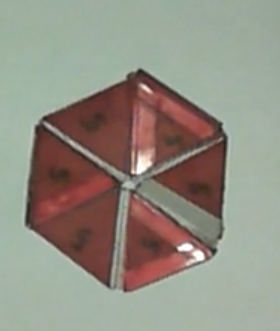
\includegraphics[scale=0.3]{/video/inerte_rouge.png}, ou
			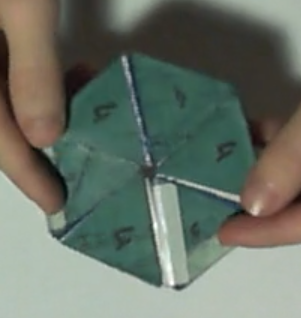
\includegraphics[scale=0.3]{/video/inerte_vert.png}
			\end{figure}
		\end{center}
		\end{frame}
		
		\begin{frame}{(Démonstration)}
		\begin{center}
			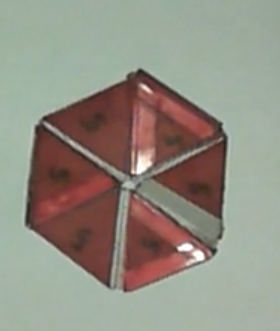
\includegraphics[scale=0.27]{/video/inerte_rouge.png}
			\Large{$\longrightarrow$}
			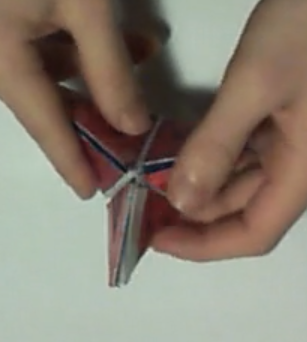
\includegraphics[scale=0.27]{/video/flexe_rouge_bleu_deb.png} \Large{$\downarrow$}\\
			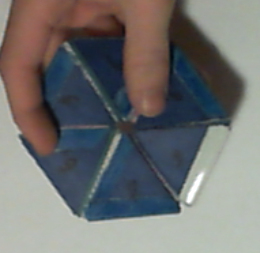
\includegraphics[scale=0.32]{/video/inerte_bleu.png}
			\Large{$\longleftarrow$}
			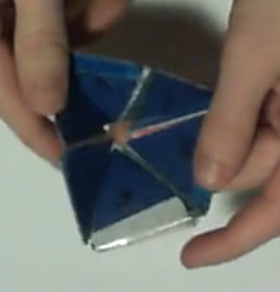
\includegraphics[scale=0.27]{/video/flexe_rouge_bleu_fin.png}\\
			\LARGE{FLEXE}
			
		\end{center}
		\end{frame}
		
		\begin{frame}
		\begin{center}
			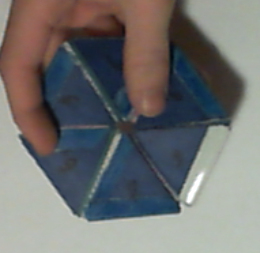
\includegraphics[scale=0.3]{/video/inerte_bleu.png}
			\Large{$\longrightarrow$}
			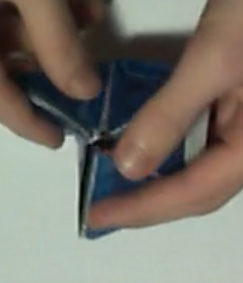
\includegraphics[scale=0.35]{/video/flexe_bleu_rose_deb.png} \Large{$\downarrow$}\\
			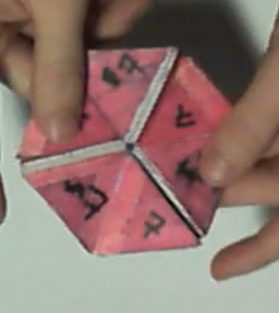
\includegraphics[scale=0.3]{/video/inerte_rose.png}
			\Large{$\longleftarrow$}
			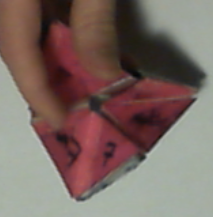
\includegraphics[scale=0.45]{/video/flexe_bleu_rose_fin.png}\\
			\LARGE{FLEXE}
		\end{center}
		\end{frame}
		
		\begin{frame}{(Démonstration)}
		\begin{center}
			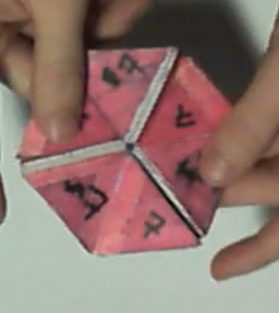
\includegraphics[scale=0.3]{/video/inerte_rose.png}\Large{$\longrightarrow$}
			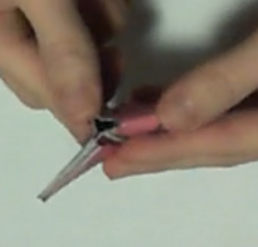
\includegraphics[scale=0.3]{/video/blocage_rose.png}\\
			\LARGE{BLOCAGE}
		\end{center}
		\end{frame}
		
		\begin{frame}{(Démonstration)}
			METTRE 3 4 PHOTOS DE FLEXAGONES POUR MONTRER CE QU'IL SE PASSE\\
			IL FAUDRA BIEN SÛR PLUSIEURS FRAME !!!!!!
		\end{frame}
		
		\begin{frame}{Ajout de faces}
		
		\begin{center}
		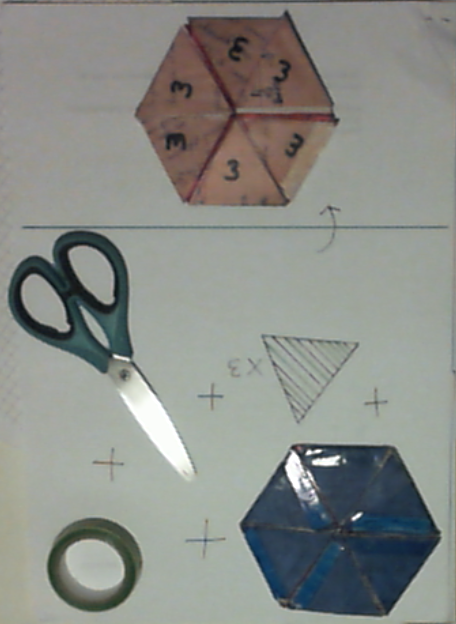
\includegraphics[scale=0.3]{outils_ajout_face.png}
		\end{center}
		\end{frame}
		
		\subsection{Objectifs}
		\begin{frame}{Objectifs}
			Comment programmer un logiciel créant les patrons d'hexaflexagones?
		\end{frame}


	\section{Préliminaire}

		\subsection{Représentations}

		\subsubsection{Patrons}
		\begin{frame}{Patrons}
			L'objet physique
			\begin{figure}
				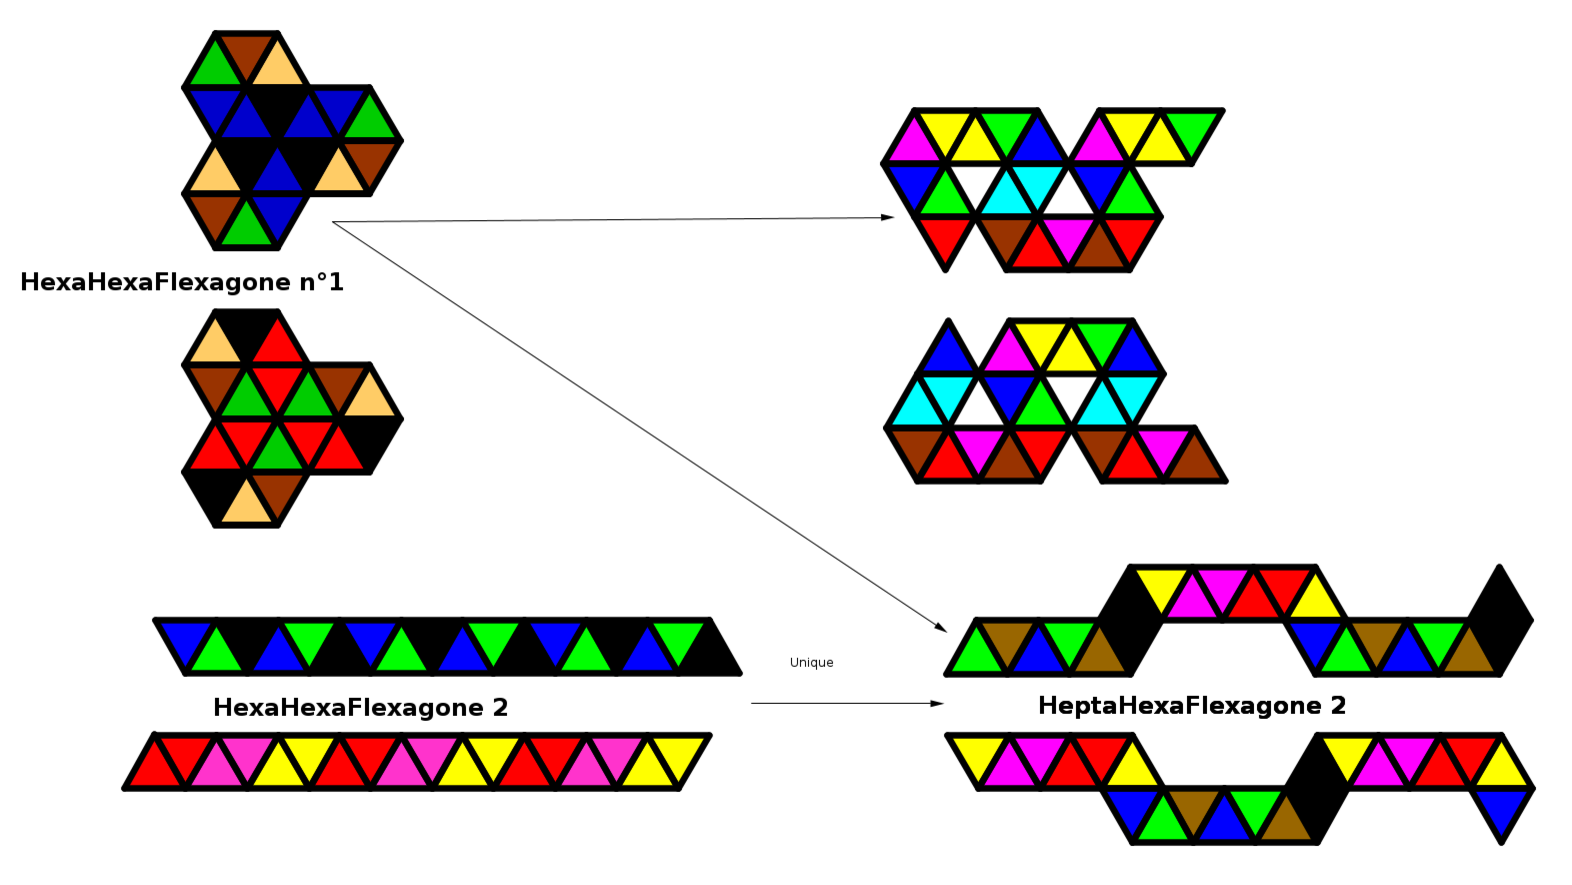
\includegraphics[scale=0.19]{exemples_patrons.png}
			\end{figure}
		\end{frame}

		\begin{frame}{Problèmes}
			Pratique ni pour la théorie ni à représenter en machine à priori.\\
			C'est pourtant ce qu'on cherche à construire.\\
			$\longrightarrow$ Représentations plus abstraites?
		\end{frame}
				
		\subsubsection{Graphes}
		\begin{frame}{Tuckerman Traverse}
			Graphe des positions du flexagone
			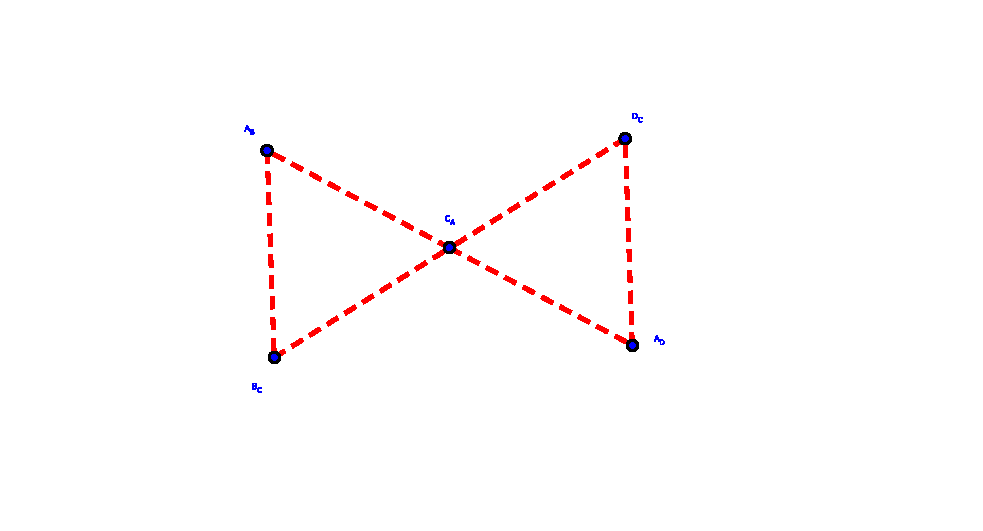
\includegraphics[scale=0.6]{TT_graphe_4.eps}\\
			Chaque sommet est un couple (couleurdevant, couleurderrière),\\
			Deux sommets sont liés $\Leftrightarrow$ On peut passer de l'un à l'autre en un flexe.\\
			Souvent appelé TT pour "Tuckerman Traverse" en l'hommage de Bryant Tuckerman.
		\end{frame}		
		
		\begin{frame}{Triangulations}
			Graphe d'adjacence des faces (couleurs) du flexagone:
			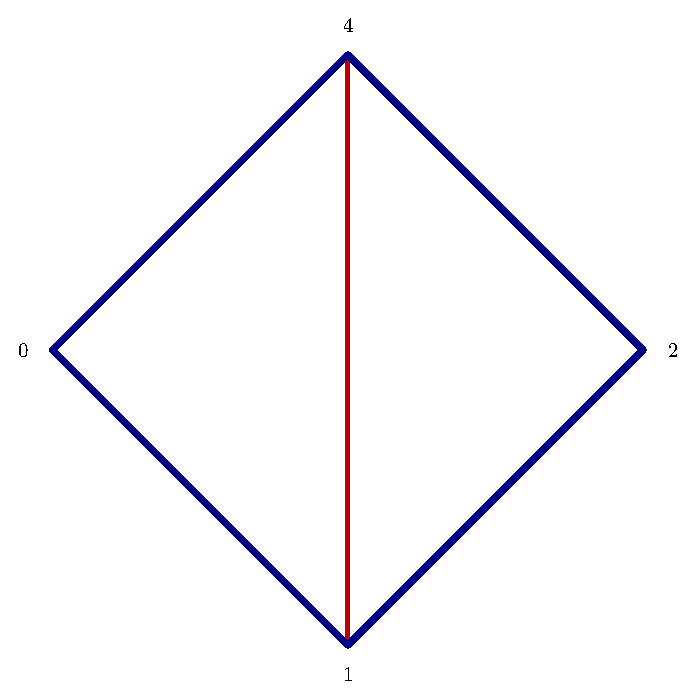
\includegraphics[scale=0.3]{triangu_4.eps}\\
			Chaque sommet est une couleur.\\
			Deux sommets sont liés $\Leftrightarrow$ Les deux couleurs sont visibles simultanément.\\
			Représentation des flexagones par des triangulation de polygones (TdP).
		\end{frame}
		
		\subsection{Dénombrement}
		\begin{frame}{Nombres de Catalan}
			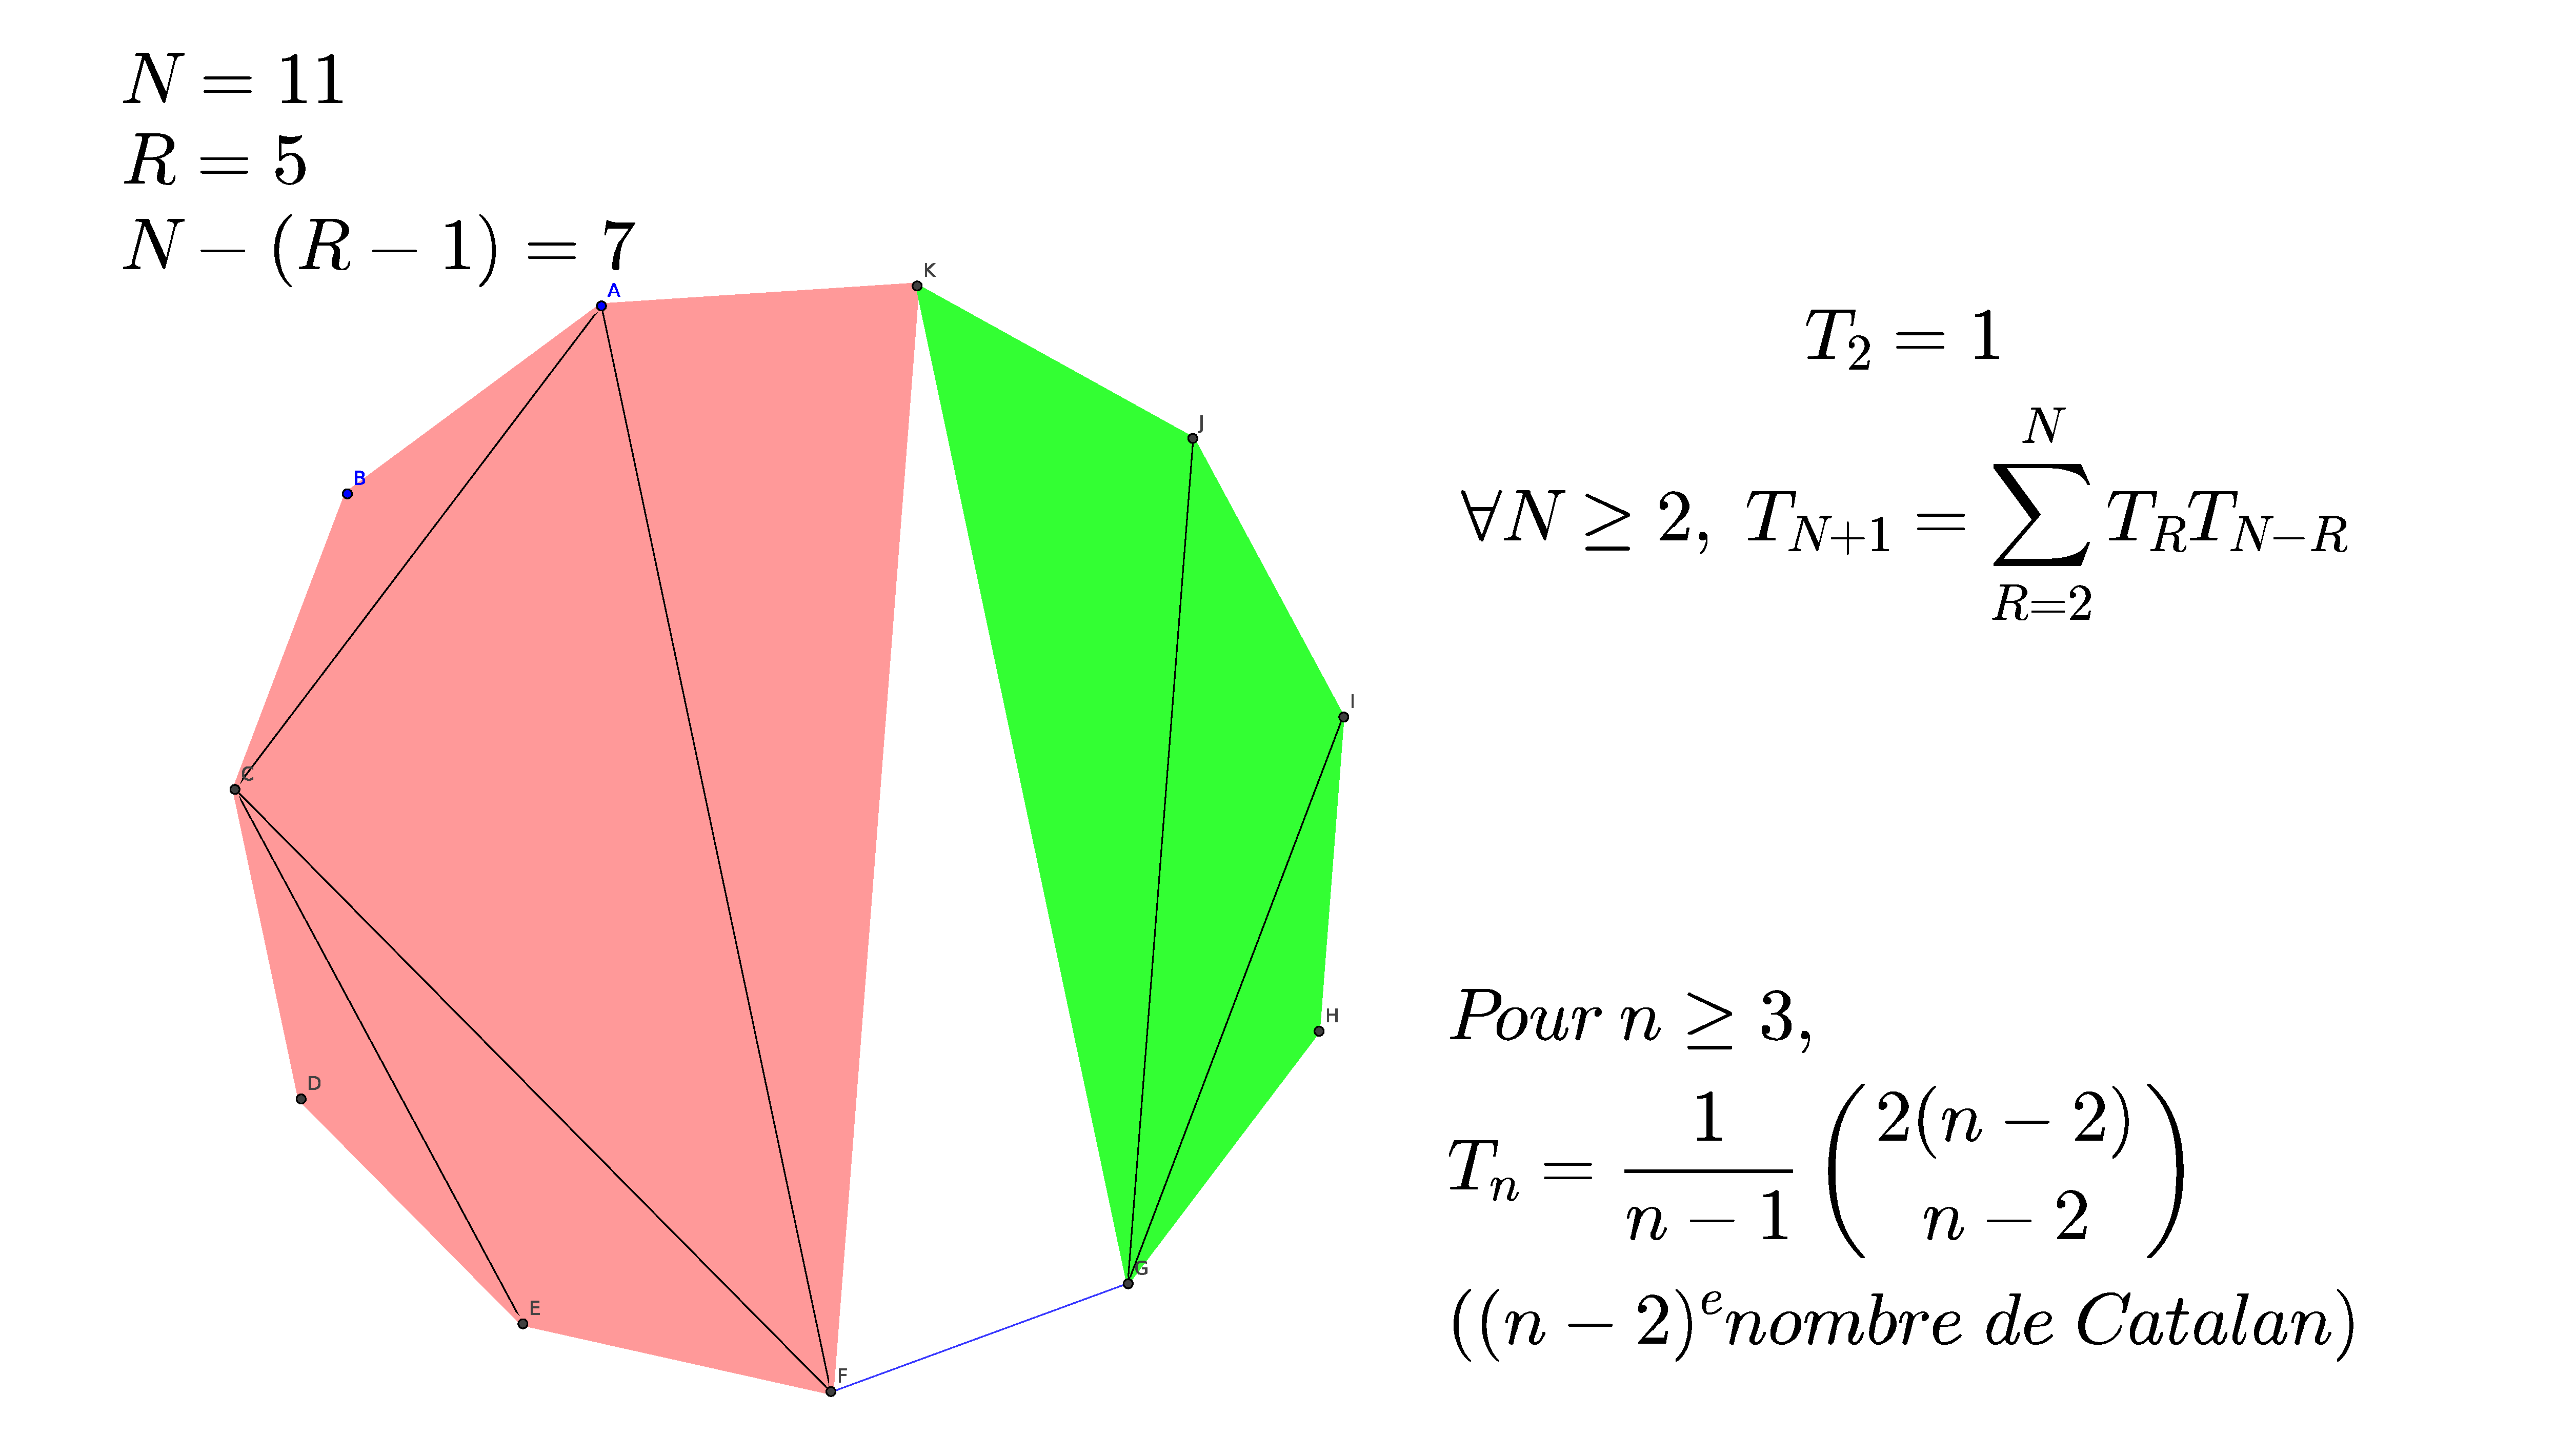
\includegraphics[scale=0.15]{nombres_catalans.eps}
		\end{frame}
		\begin{frame}{Groupe diédral}
			Le groupe diédral d'ordre $n\geqslant 3$ est le groupe d'invariance du $n-gone$ régulier.\\
			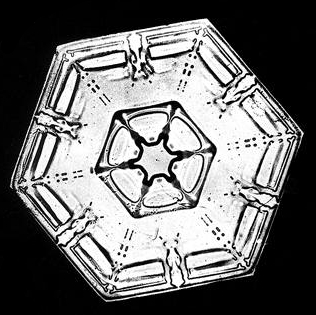
\includegraphics[scale=0.22]{snowflake.jpg}
		\end{frame}
		
		\begin{frame}{Action de groupe}
			\begin{definition}[Action de groupe]
			Pour un ensemble X, un groupe G, une action de G sur X est un morphisme de groupes
			$\phi: G \rightarrow \mathfrak{S}_{X}$.\\
			Relation d'équivalence associée:
			\[
				\forall x,y \in X,\; x \mathcal{R} y \Leftrightarrow \exists g \in G, x=\phi(g)(y)
			\]
			On note $X/G$ le quotient $X/\mathcal{R}$.
			\end{definition}
			
			On étudie les triangulations du n-gone régulier sous l'action de $D_{n}$.
		\end{frame}
		
		\begin{frame}{Lemme de Burnside}
			\begin{theorem}[Lemme de Burnside]
				G un groupe fini, X un ensemble fini, alors
				\[
				|X/G| = \frac{1}{|G|}\sum_{g\in G}{|Fix(g)|}
				\]
				Où $Fix(g) = \{x\in X, g(x) = x\}$.
			\end{theorem}
		\end{frame}
		
		\begin{frame}{Application au dénombrement}
			Avec $G=D_{n}=\langle\tau,\rho\mid \tau^{2}=\rho^{n}=(\tau\rho)^{2}=1\rangle$
			\[
				|X/D_{n}| = \frac{1}{2n}\sum_{k=0}^{n}|Fix(\rho^{k})|+|Fix(\rho^{k}\tau\rho^{-k})|
			\]
		\end{frame}
		\begin{frame}{Cas des rotations}
		\begin{figure}[1]
		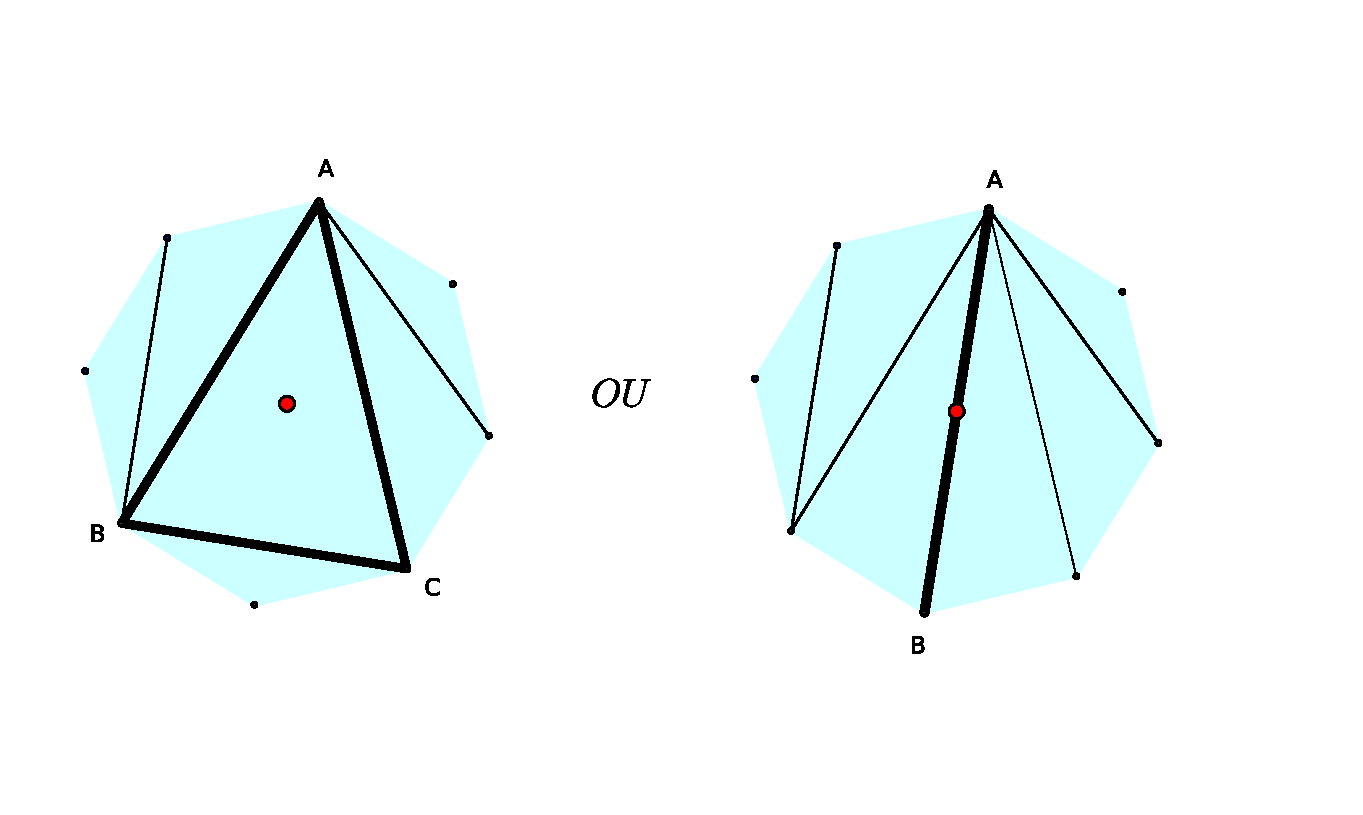
\includegraphics[scale=0.45]{invariances_rotation.eps}
			\caption{Seules les rotations d'angle $\pi$ ou $2\pi/3$ peuvent laisser invariante une triangulation}
			\end{figure}
		\end{frame}
		
		\begin{frame}{Cas des rotations}
			On note $C_{n}=\frac{1}{n+1}\binom{2n}{n}$ si $n\in\mathbb{N}$, $0$ sinon. 
 le $n^{e}$ nombre de Catalan.\\
			On cherche les éléments fixés par $\rho^{n/2}$ et $\rho^{n/3}$.\\
			Pour $\rho^{n/2}$: $\frac{n}{2}$ axes de symétrie et $C_{n/2-1}$ triangulations pour chacun.\\
			$\longrightarrow |Fix(\rho^{n/2})|=\frac{n}{2}C_{n/2-1}$\\
			De même, $|Fix(\rho^{n/3})|=\frac{n}{3}C_{n/3-1}$
		\end{frame}
	
		\begin{frame}{Finalement}
		On a compté nos flexagones, pour $n>2$:
		{\large
		\[
			|F_{n}| = \frac{1}{2n}C_{n-2} + \frac{1}{4}C_{n/2-1} + \frac{1}{2}(C_{(n-1)/2}+C_{n/2-1}) + \frac{1}{3}C_{n/3-1}
		\]
		}
		\begin{wrapfigure}{l}{0.6\textwidth}
			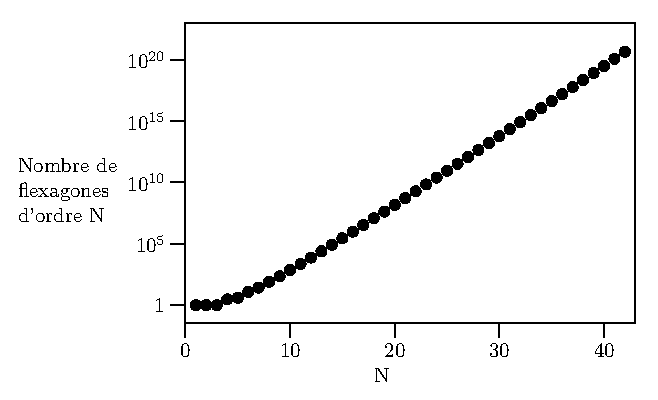
\includegraphics[scale=0.6]{nombre_flexagones.eps}
		\end{wrapfigure}
		\begin{flushleft}
			Avec $C_{x} = 0$ si $x \not\in \mathbb{N}$.\\
		$|F_{n}| \sim \dfrac{4^{n-2}}{n^{2}\sqrt{n\pi}}$
		\end{flushleft}
	\end{frame}


	\section{Construction}
		\subsection{Représentation}
		
		\begin{frame}{Objectifs}
			\begin{itemize}
					\item Représenter et construire les TdP.
					\item Transformer ces représentations en patrons de flexagone (prêts pour l'impression).
			\end{itemize}		
		\end{frame}

		\begin{frame}{Construction des triangulations}
			Les trois premières triangulations sont uniques:
			\begin{figure}
				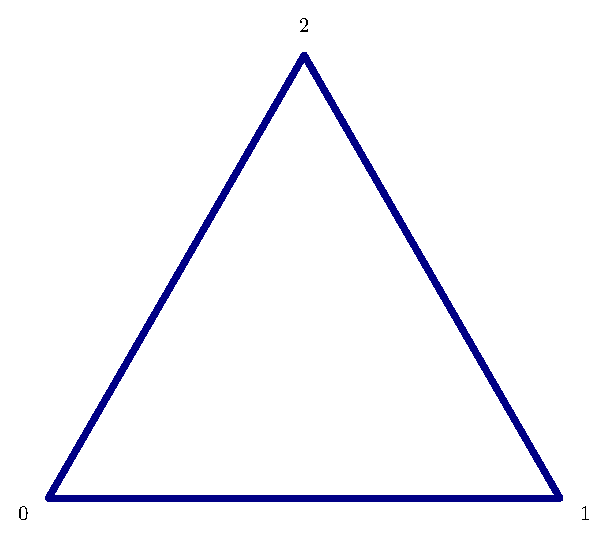
\includegraphics[scale=0.2]{triangu_3.eps}
				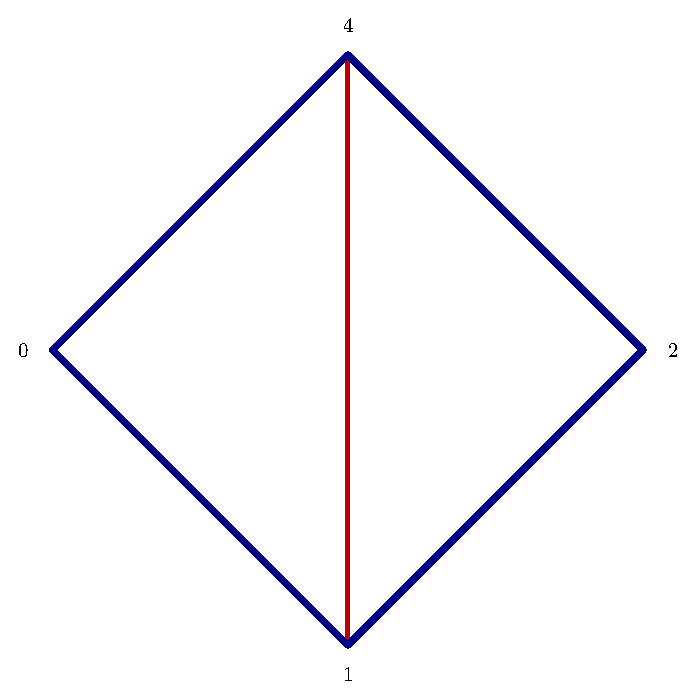
\includegraphics[scale=0.2]{triangu_4.eps}
				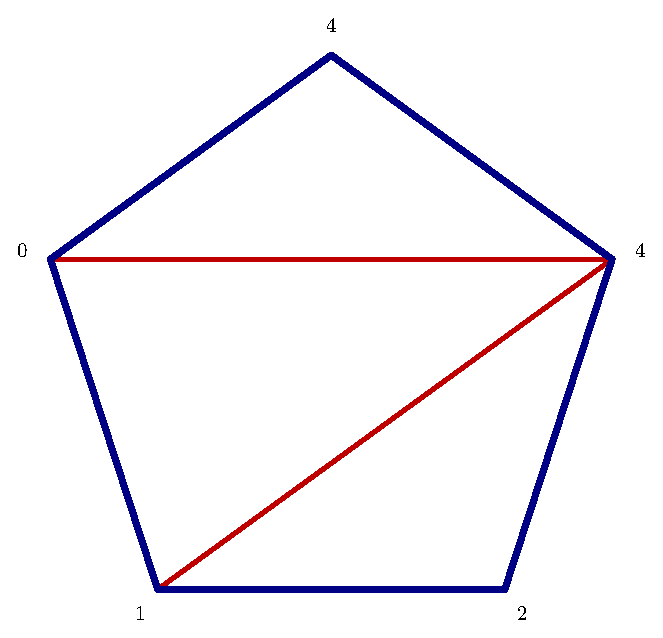
\includegraphics[scale=0.2]{triangu_5.eps}
			\end{figure}
		\end{frame}
		\begin{frame}{Construction des triangulations}
			Ajout de face: concaténation d'un triangle sur un côté du polygone
			\begin{figure}
				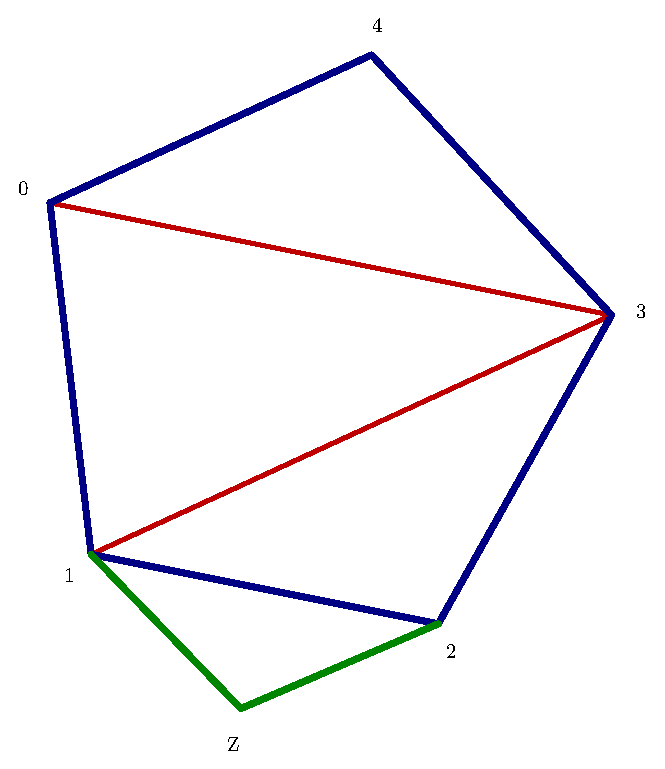
\includegraphics[scale=0.3]{exemple_triangu_ajoute_face_debut.eps}
				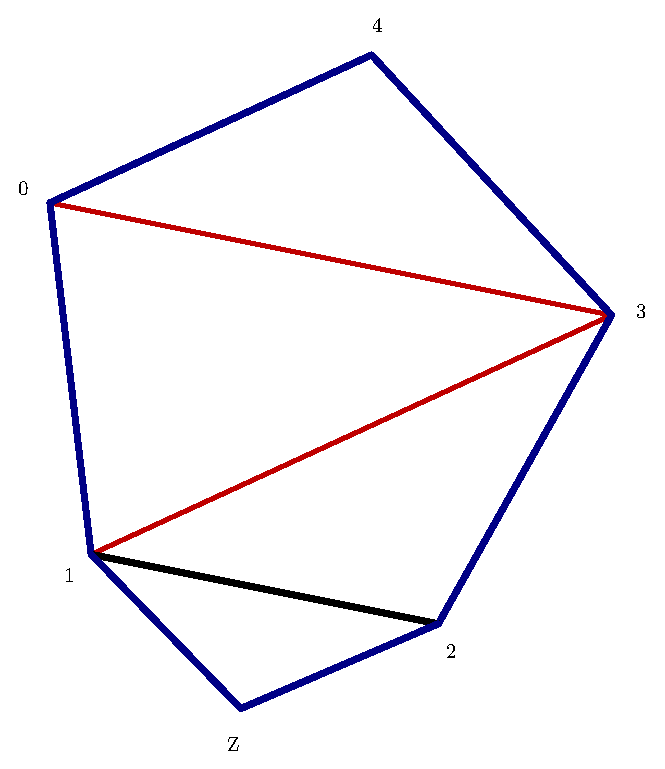
\includegraphics[scale=0.3]{exemple_triangu_ajoute_face_fin.eps}
			\end{figure}
		$\rightarrow$ Construction par récurrence des triangulations.\\
		\end{frame}
		
		\subsection{Création des patrons}
		
		\begin{frame}{Déformation}
			\begin{center}
				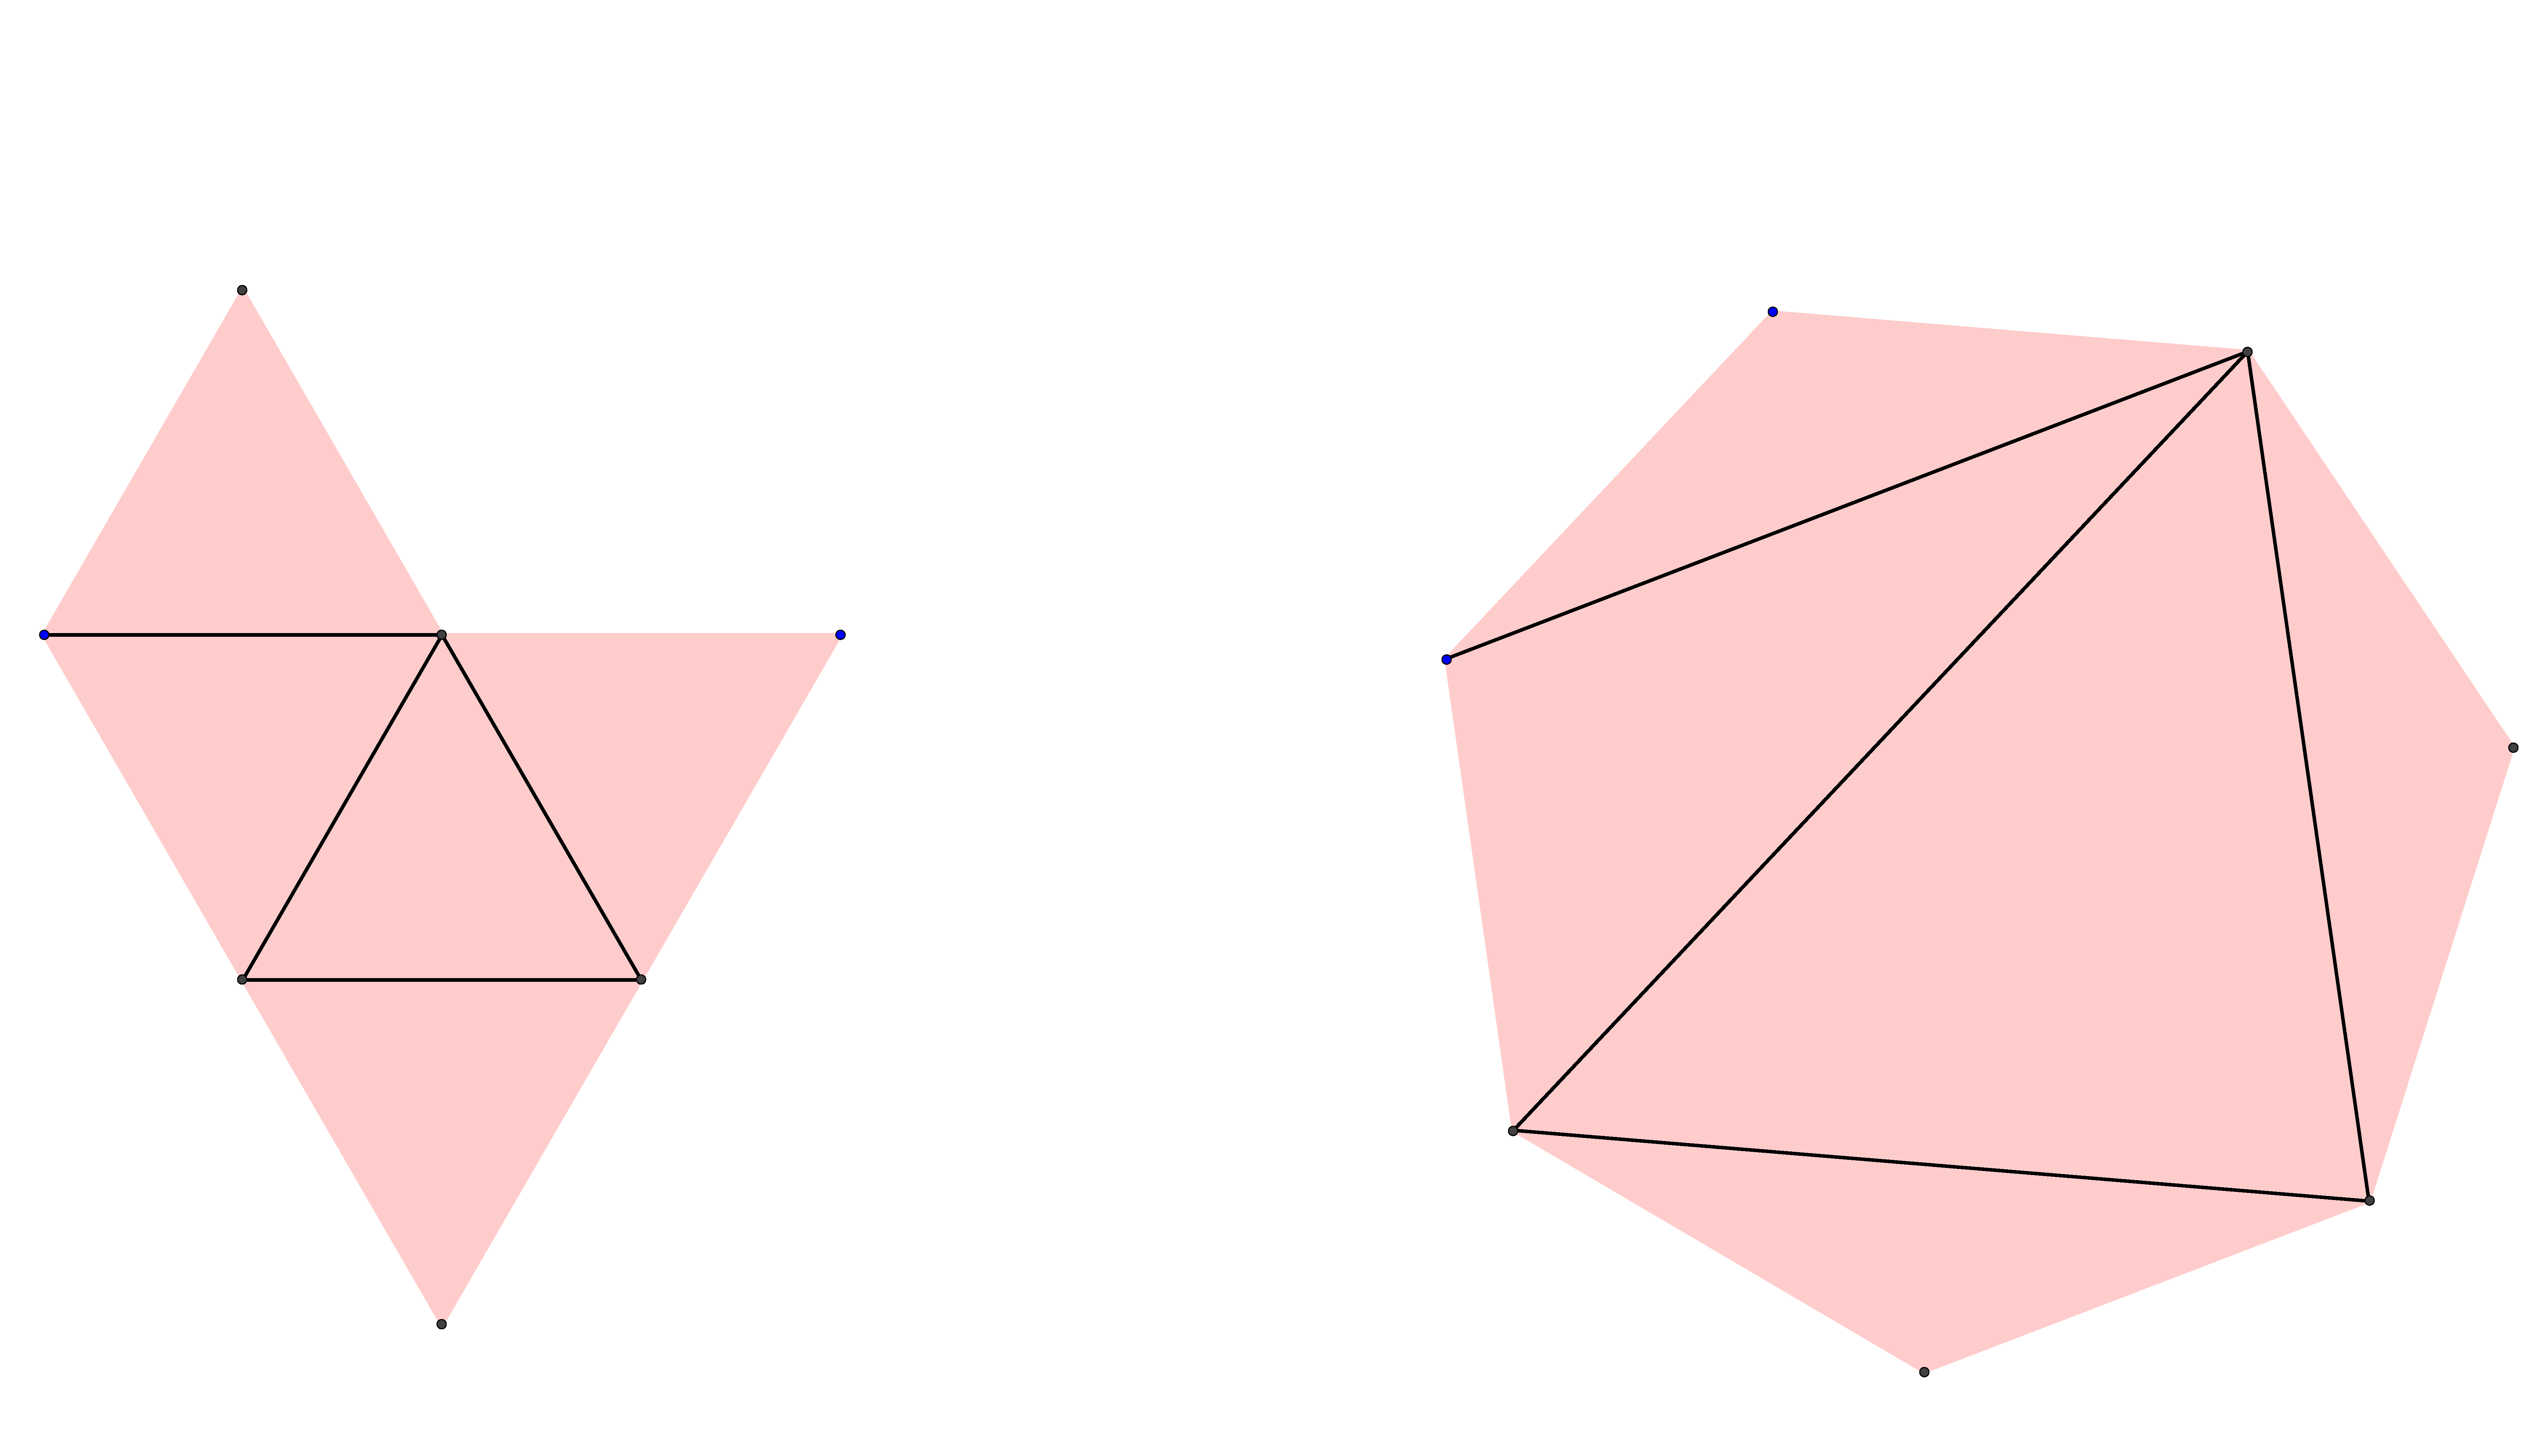
\includegraphics[scale=0.08]{equiv_tuckey_feynmann.eps}
			\end{center}
			\begin{flushleft}
				Diagramme de Tuckey
			\end{flushleft}
			\begin{flushright}
				Diagramme de Feynmann
			\end{flushright}
		\end{frame}
		
		\begin{frame}{Interprétation des diagrammes}
			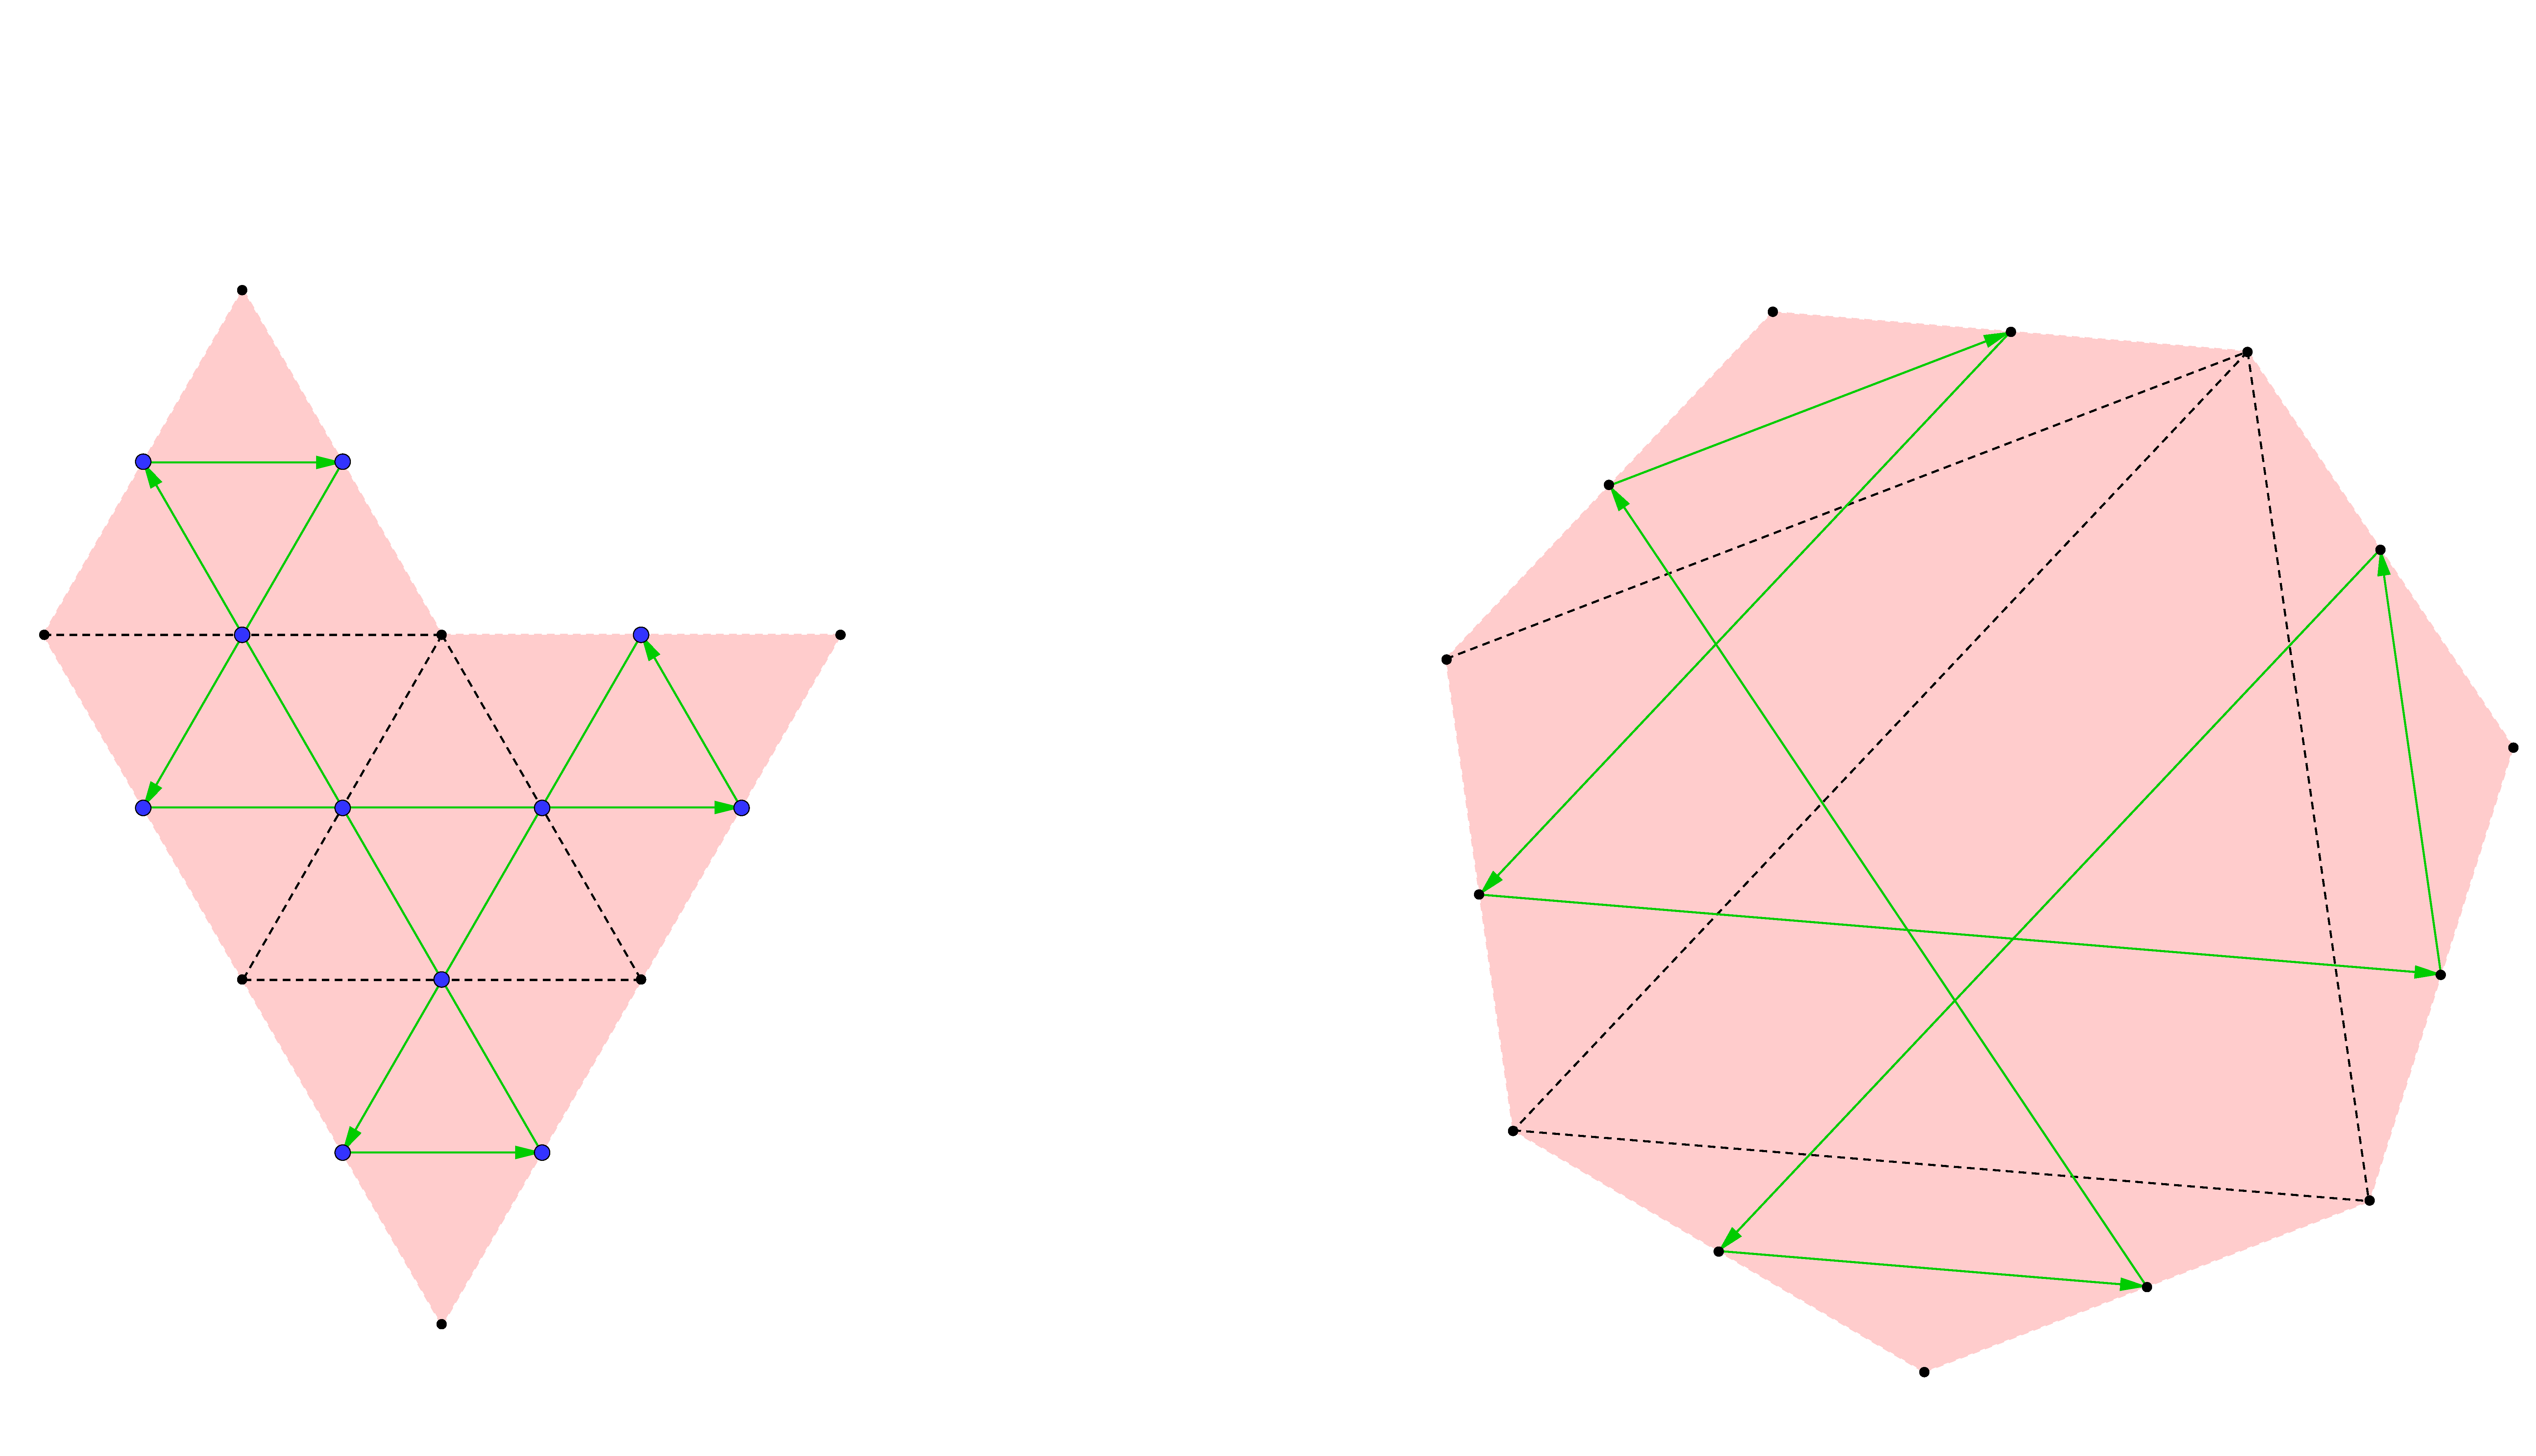
\includegraphics[scale=0.08]{conversion_tuckey_patron_1.eps}
		\end{frame}

		\begin{frame}{Interprétation des diagrammes}
			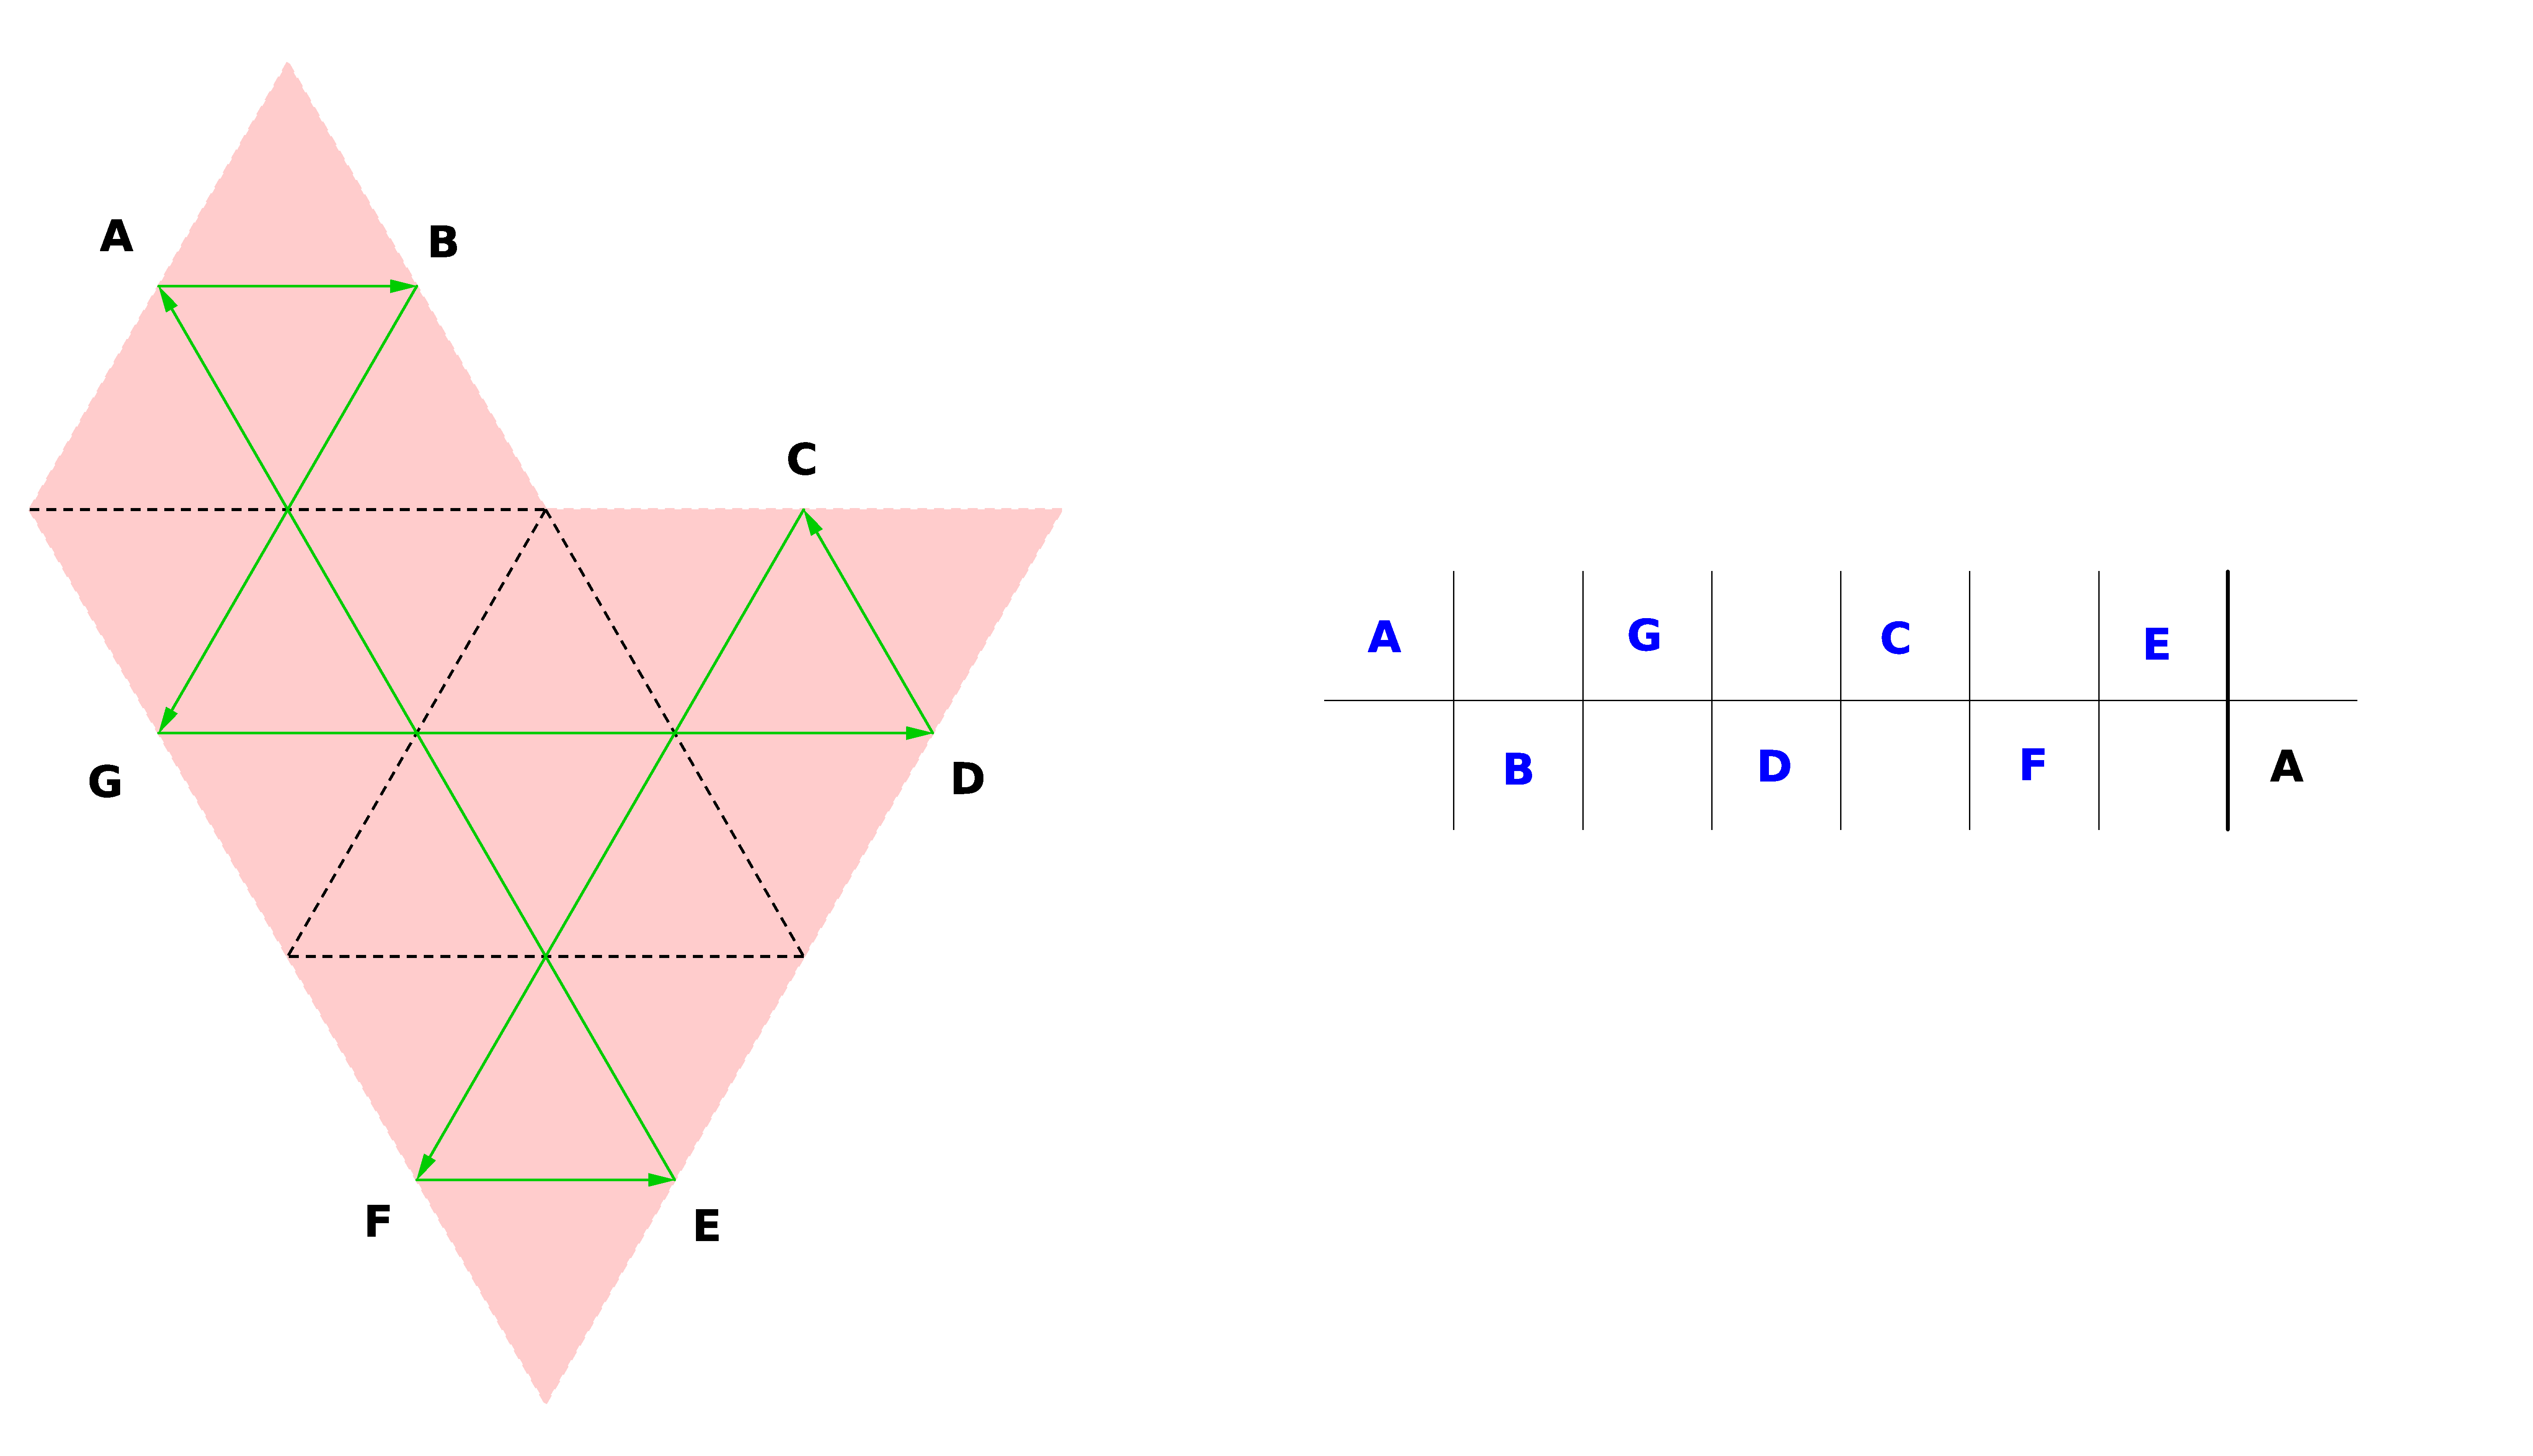
\includegraphics[scale=0.1]{conversion_tuckey_patron_2.eps}
		\end{frame}

		\begin{frame}{Interprétation des diagrammes}
			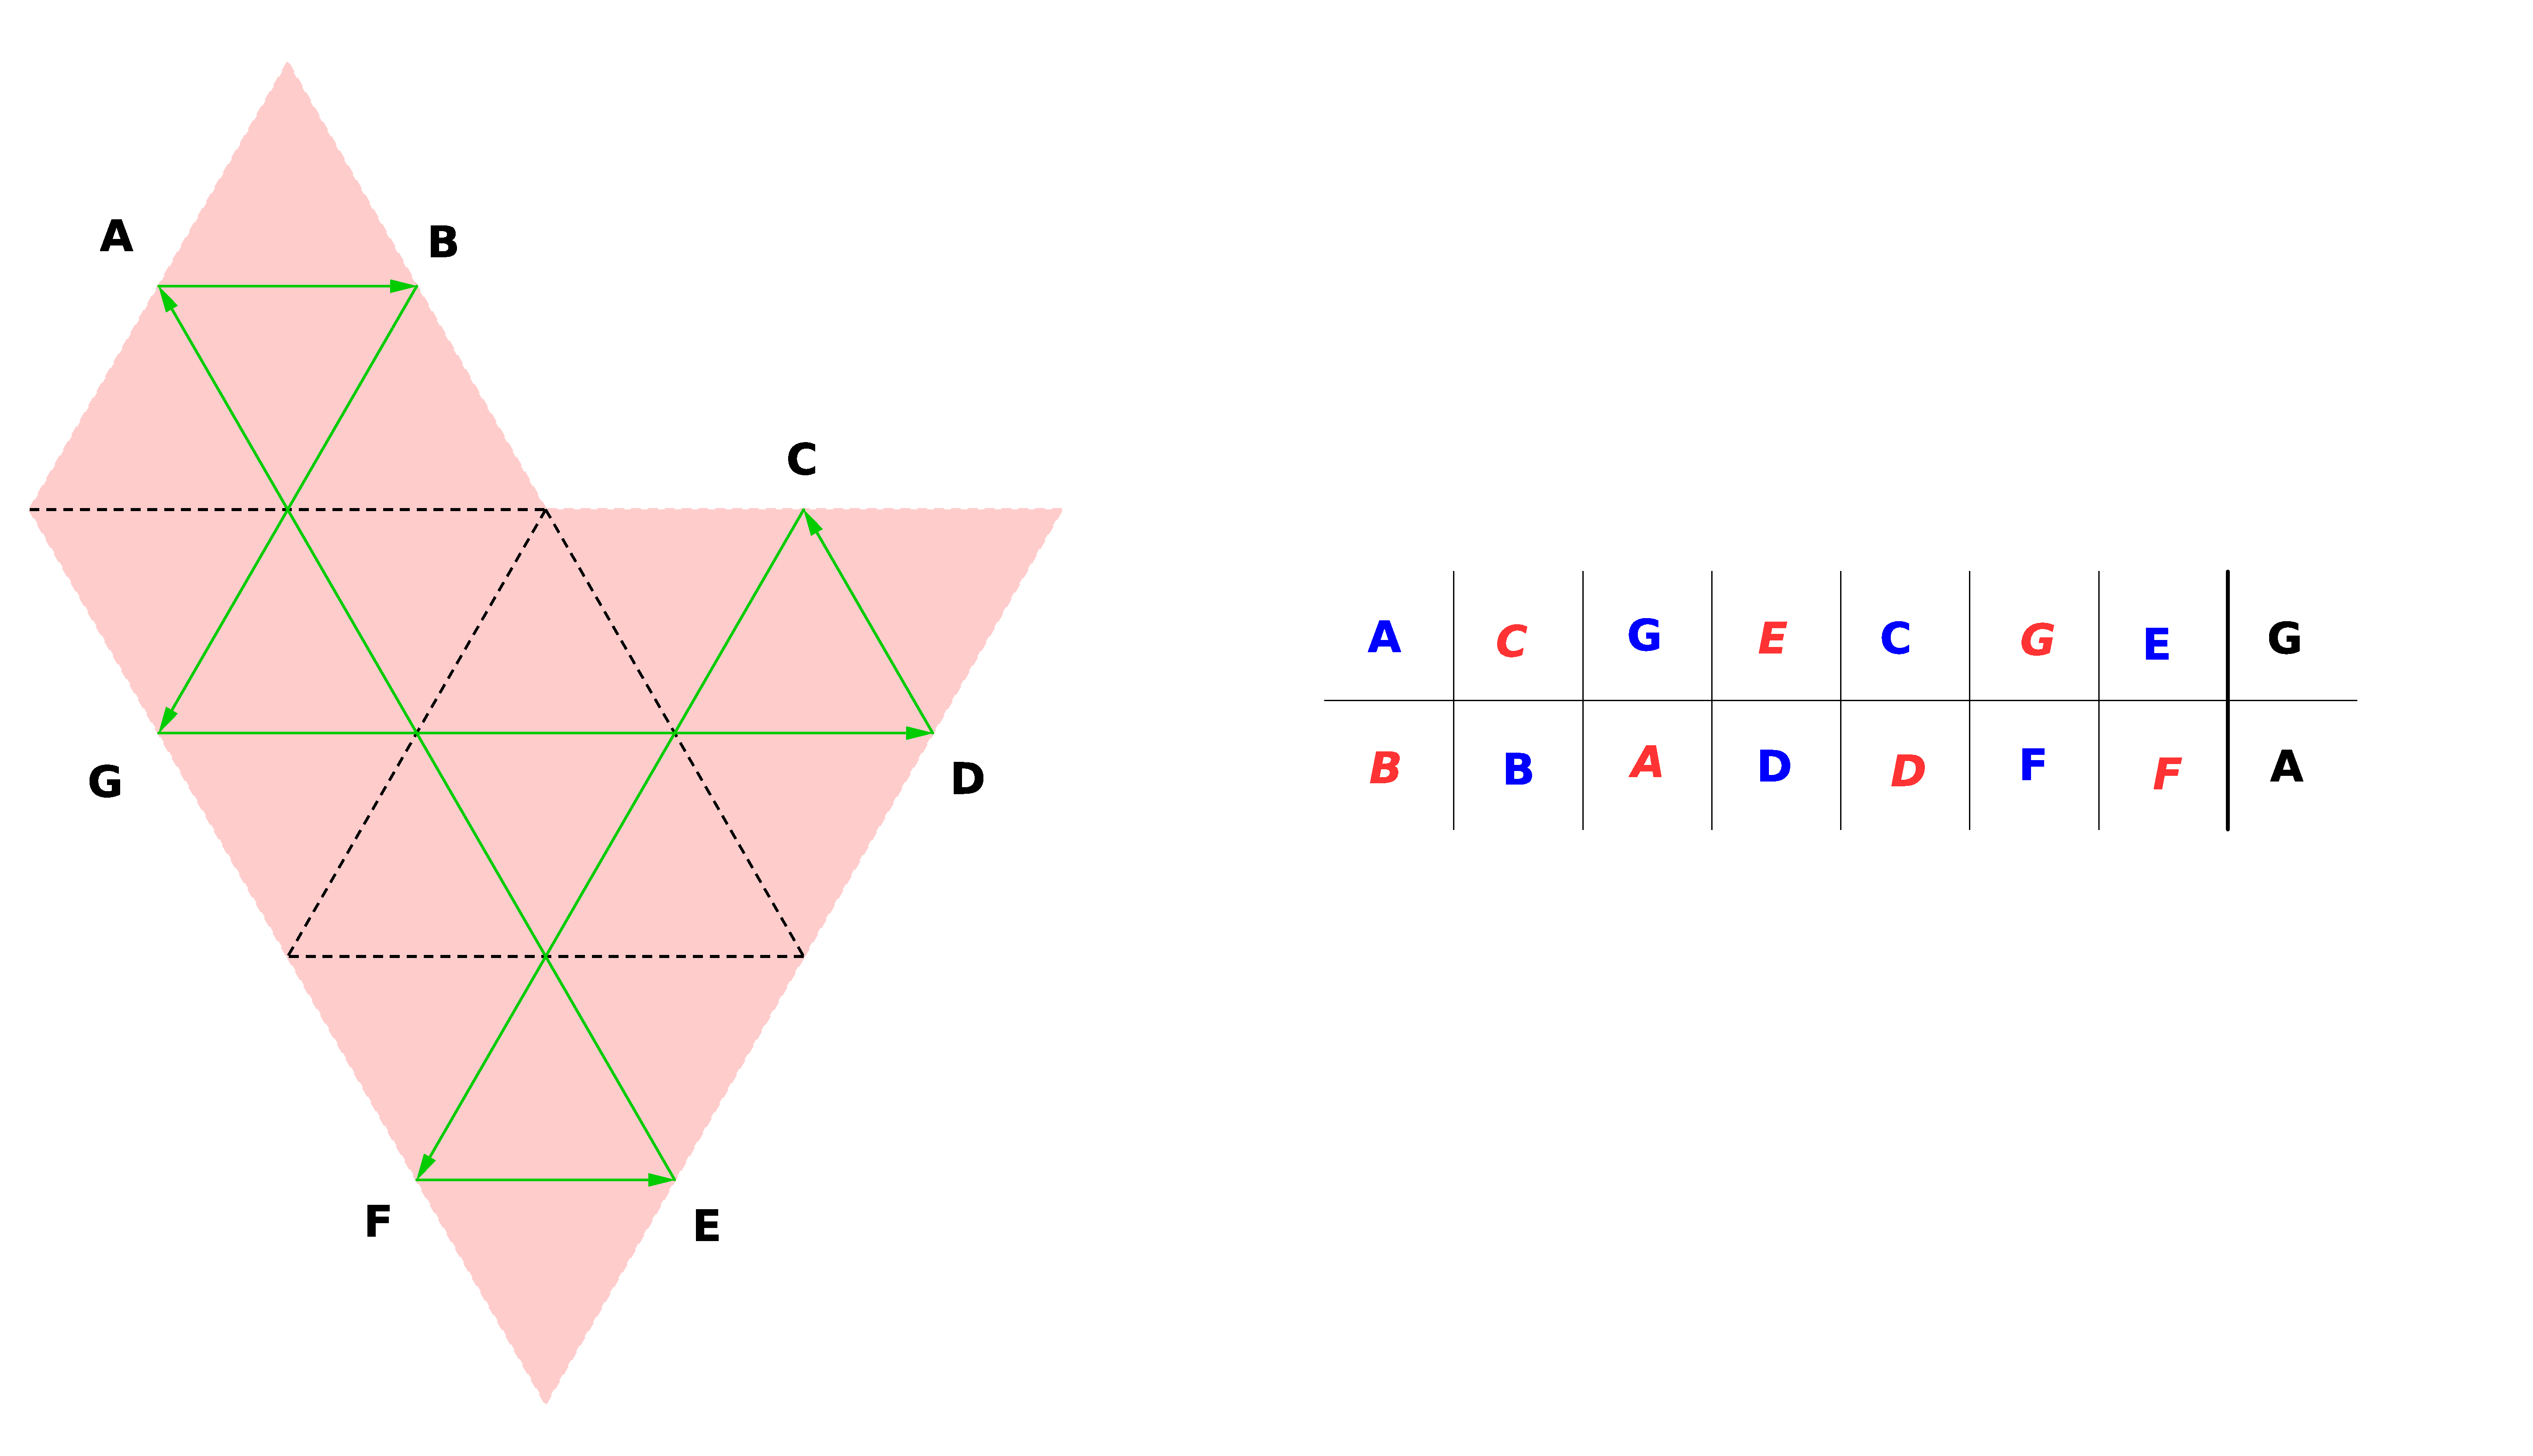
\includegraphics[scale=0.1]{conversion_tuckey_patron_3.eps}
		\end{frame}
		
		\begin{frame}{Interprétation des diagrammes}
			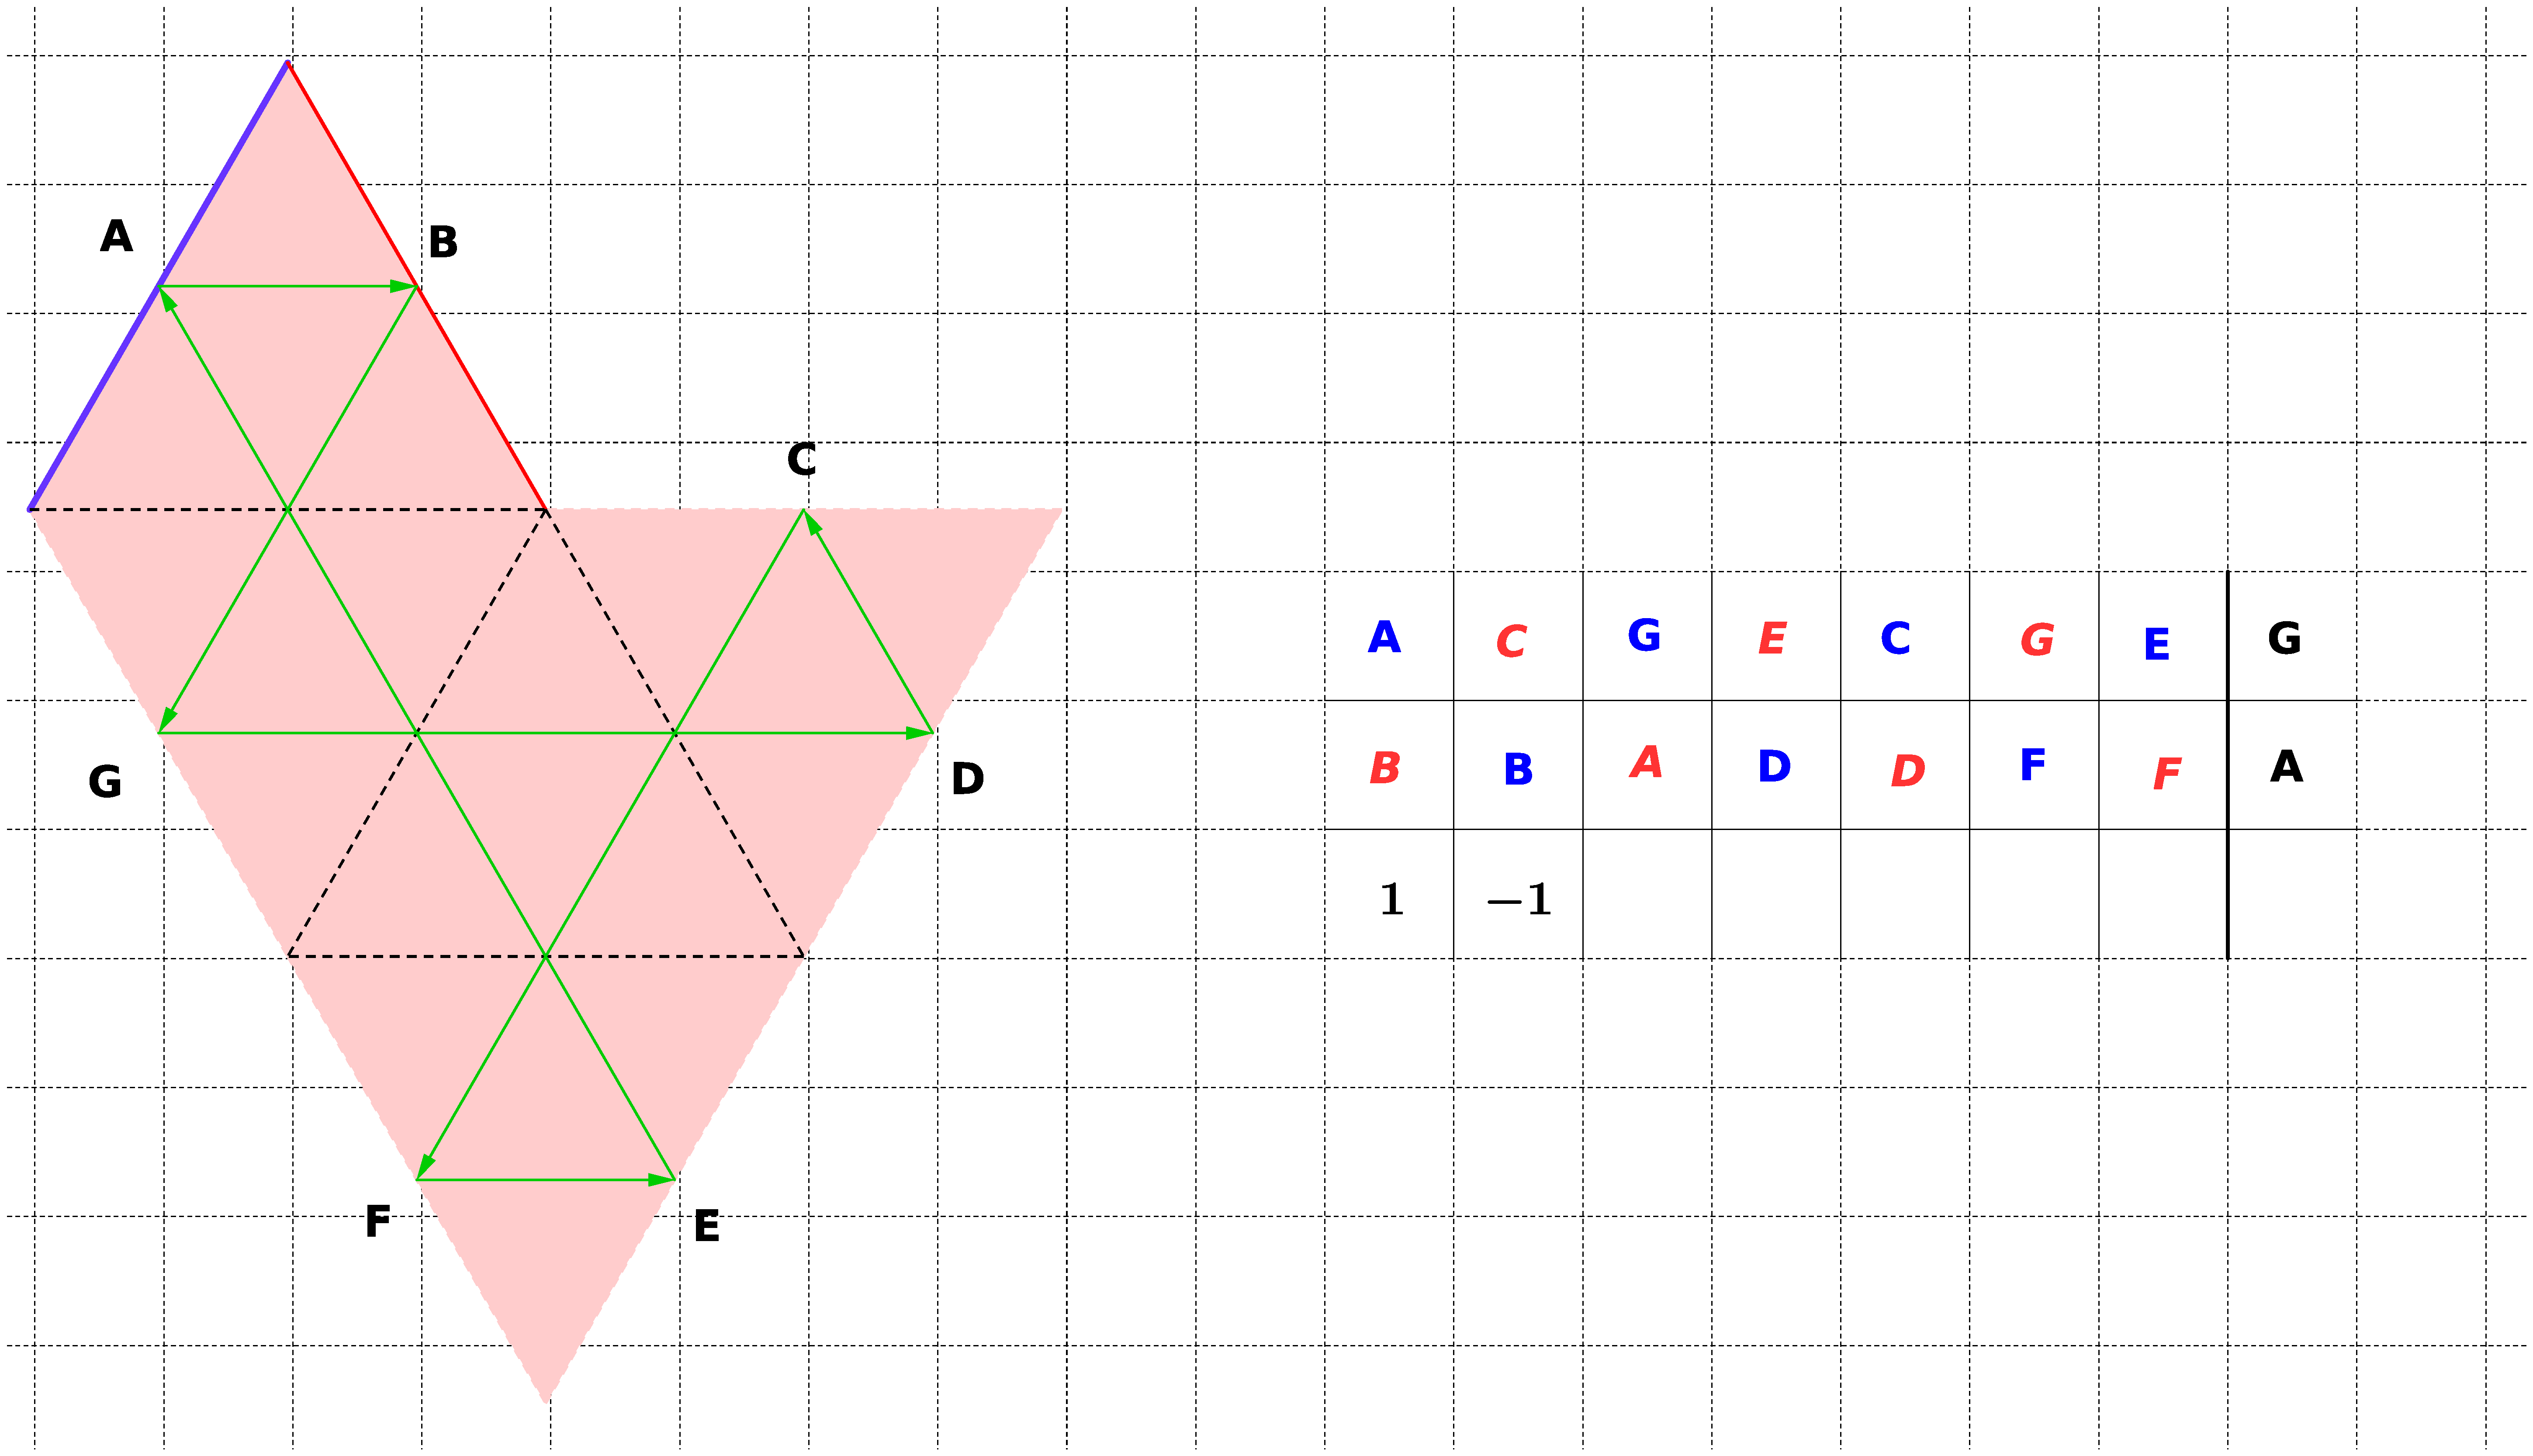
\includegraphics[scale=0.1]{conversion_tuckey_patron_4.eps}
		\end{frame}
		
		\begin{frame}{Interprétation des diagrammes}
			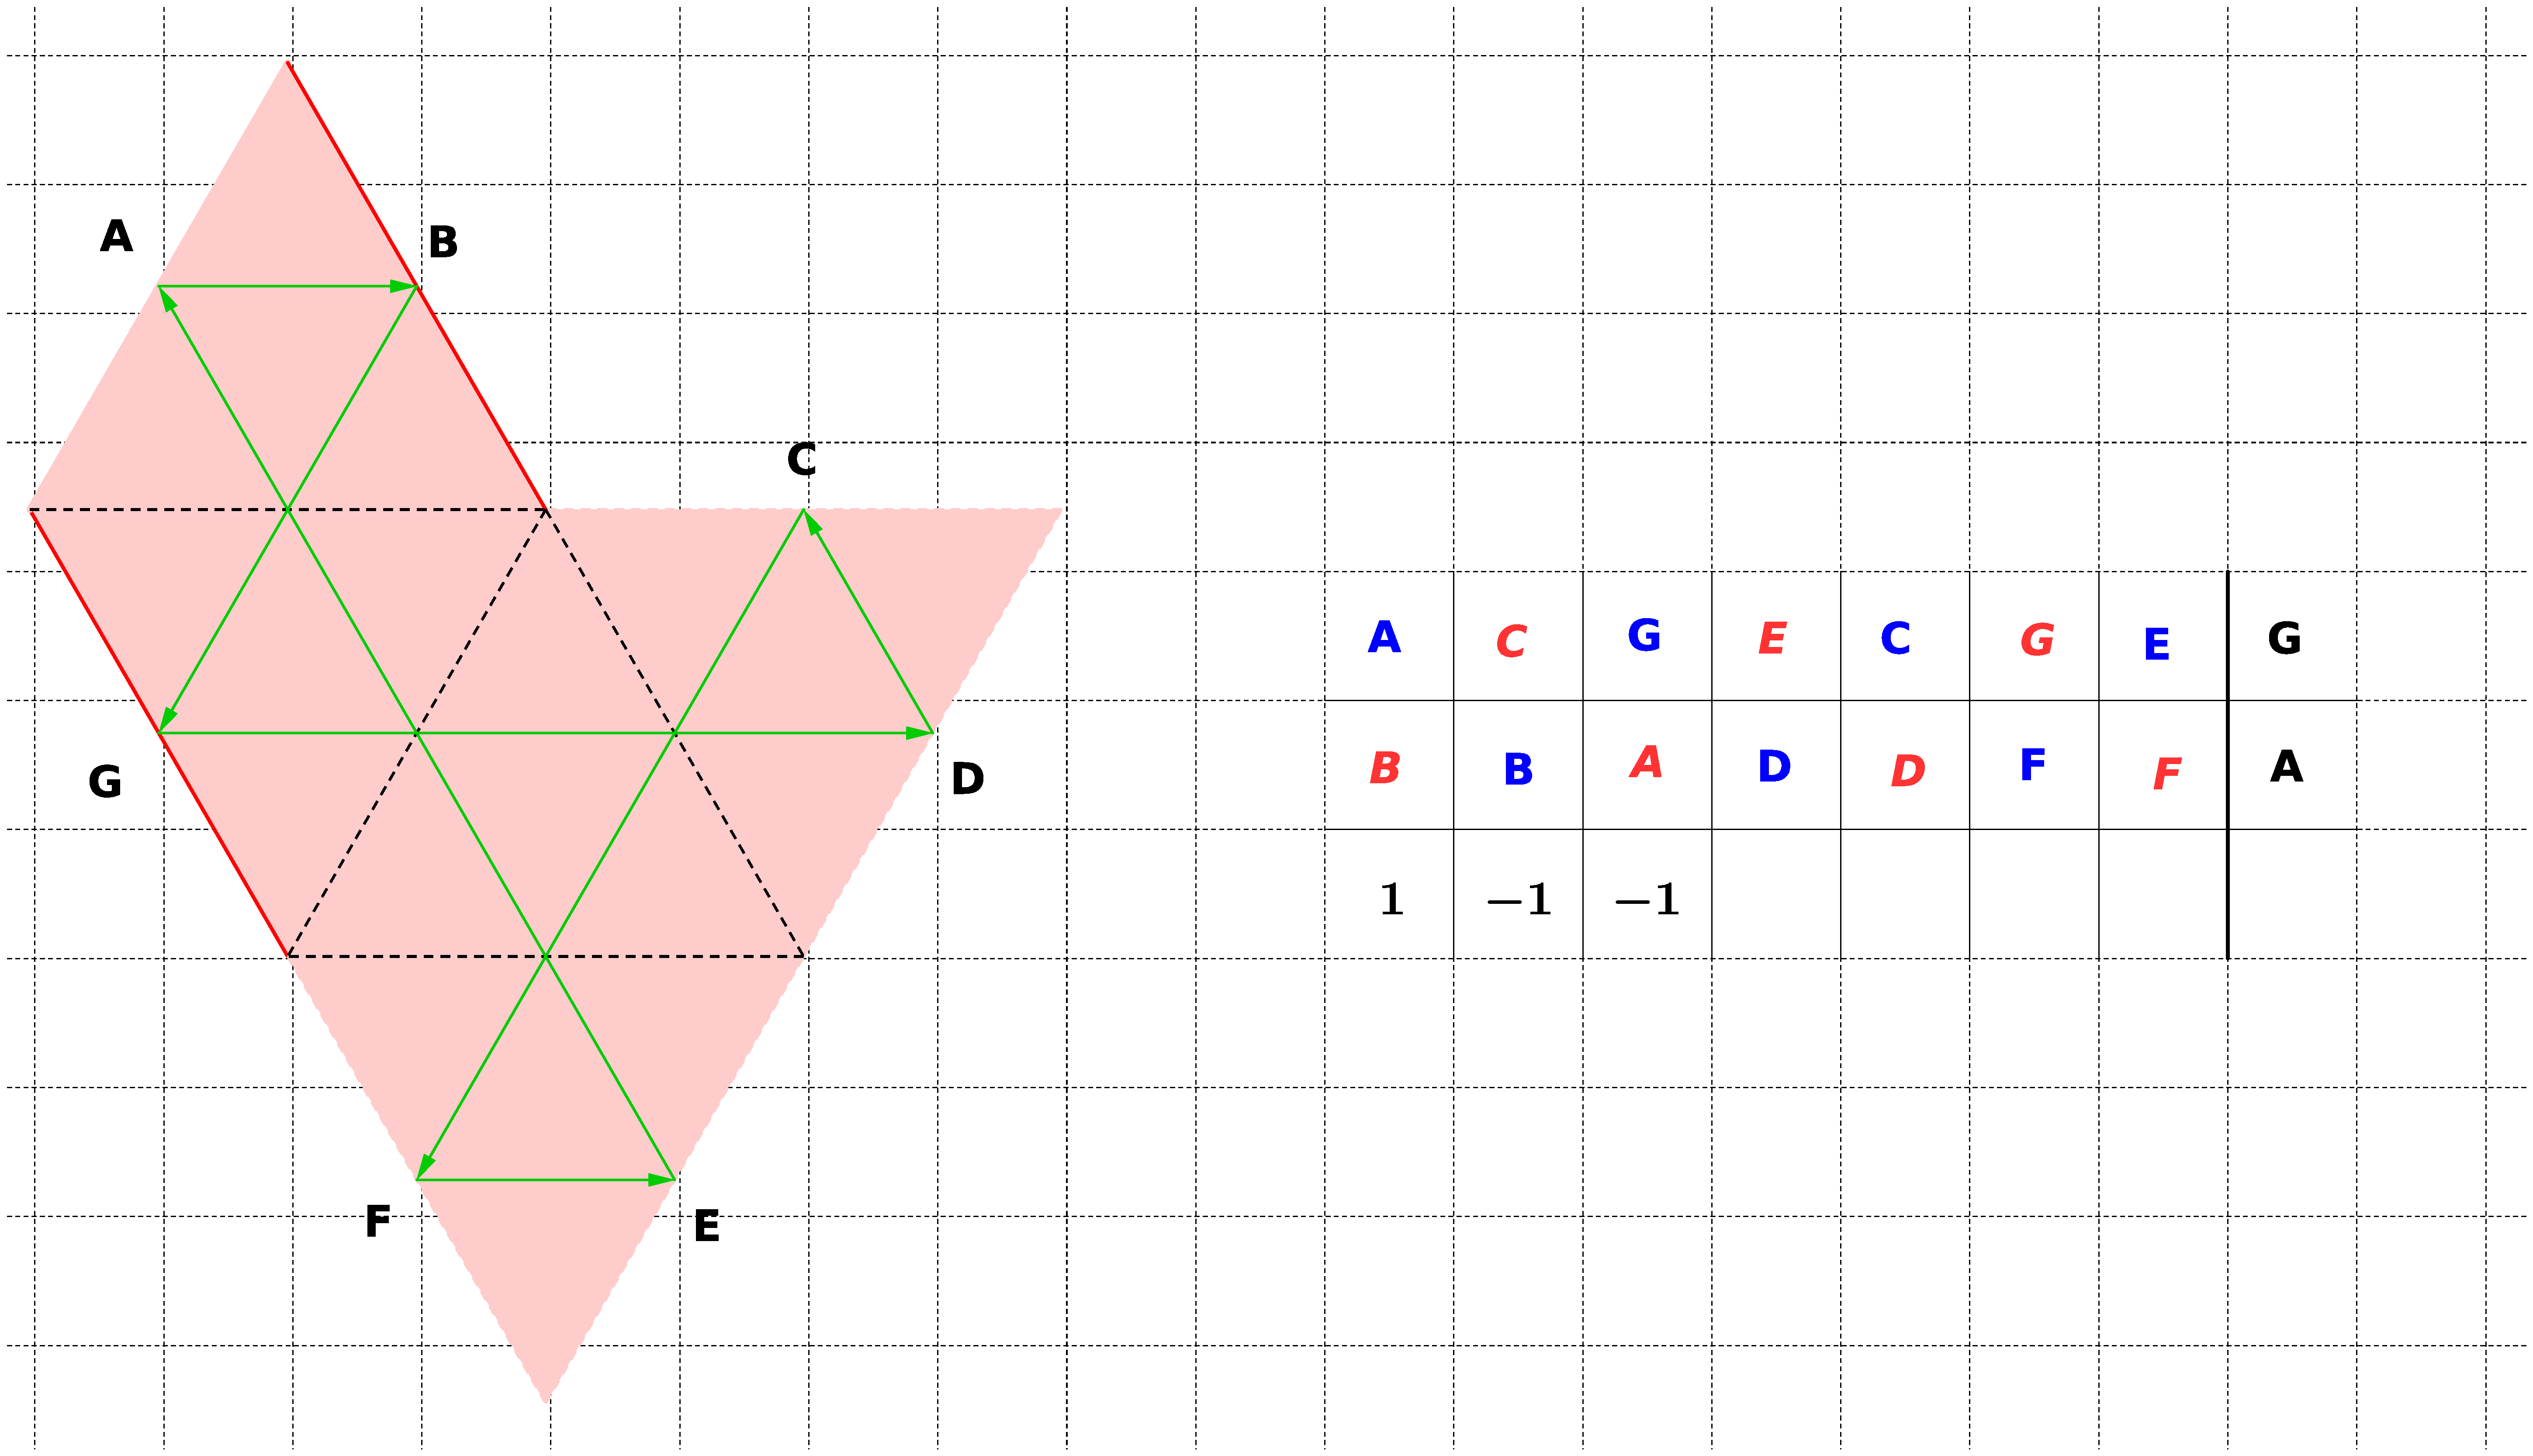
\includegraphics[scale=0.1]{conversion_tuckey_patron_5.eps}
		\end{frame}
		
		\begin{frame}{Interprétation des diagrammes}
			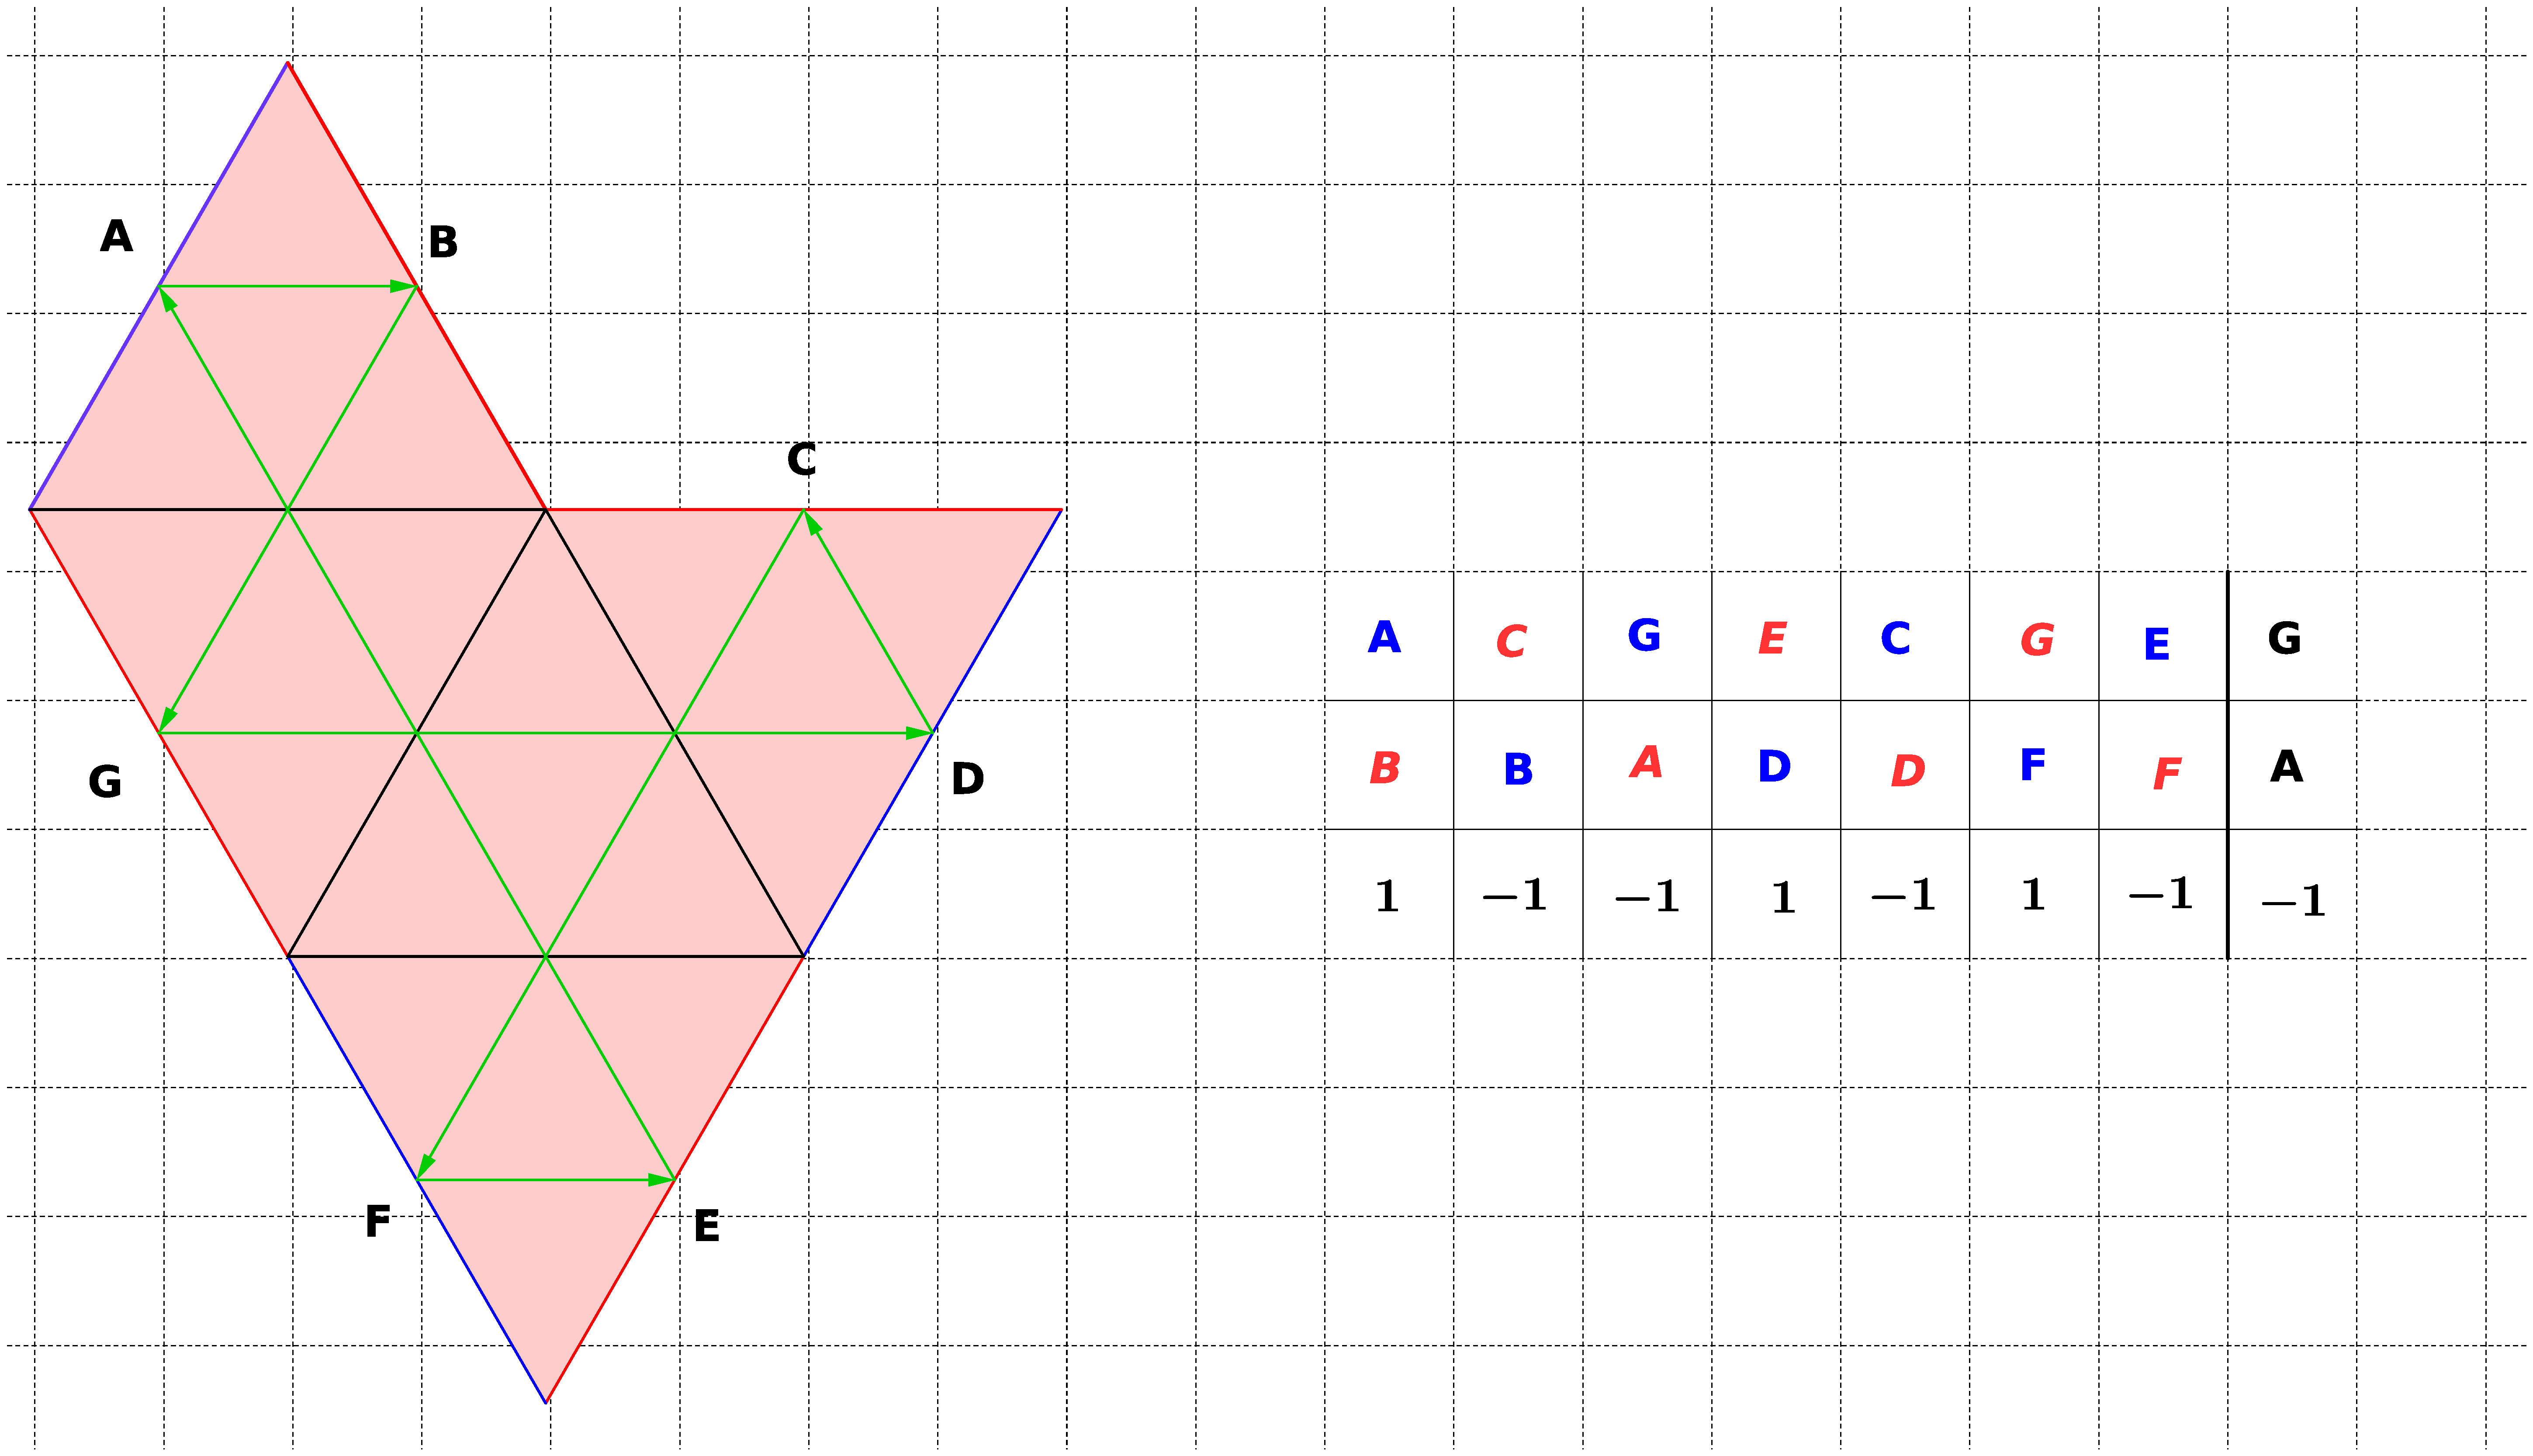
\includegraphics[scale=0.1]{conversion_tuckey_patron_6.eps}\\
			Ces triplets permettent de construire le patron de manière très efficace.
		\end{frame}
		
		\subsection{Implémentations}
		\begin{frame}{Construction en machine}
			Plusieurs idées plus ou moins abouties:\\
			\begin{enumerate}
			\item[•] Construire les triangulations puis les convertir
			\item[•] Construire directement les patrons (avec les listes de triplets)
			\item[•] Trouver d'autres représentations plus maniables.
			\end{enumerate}
		\end{frame}

		\begin{frame}{Triangulations de polygones}
		\underline{Description de graphes}:\\
			\begin{description}
			\item[$\odot$]Un entier: l'ordre du polygone/flexagone
			\item[$\odot$]Une liste de couples: les arêtes internes
			\end{description}
			\begin{figure}
				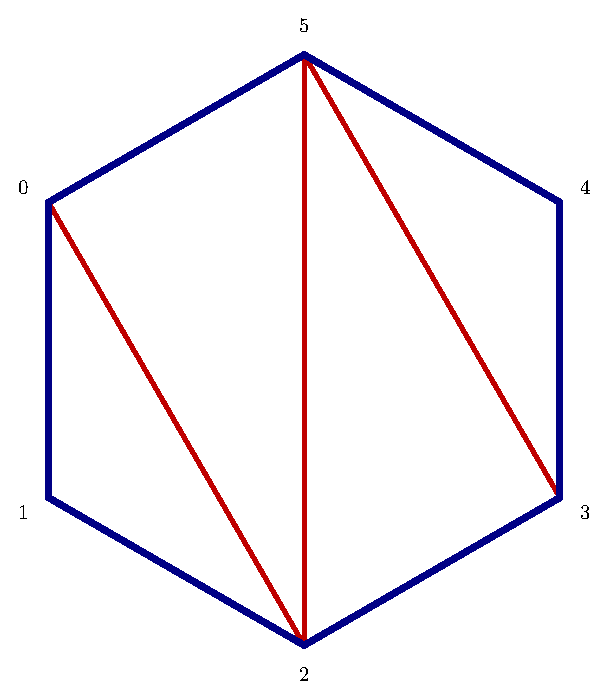
\includegraphics[scale=0.3]{exemple_6_rot.eps}\bigskip 
				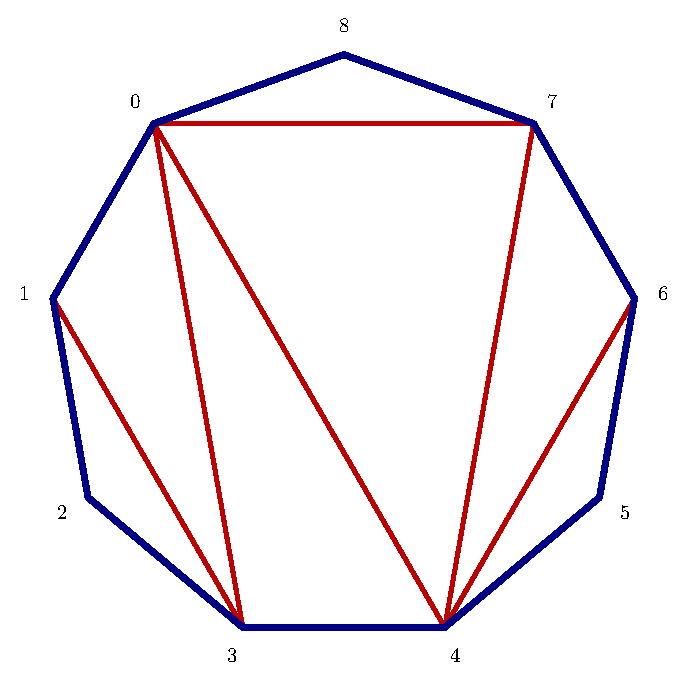
\includegraphics[scale=0.3]{exemple_triangu_9.eps}
			\end{figure}
		\end{frame}

		\begin{frame}{Construction}
			\underline{Problème}: Éviter les doublons \small{$\rightarrow$} résoudre l'isomorphisme de graphes?\\

			\underline{Solution}:Renuméroter les sommets à chaque ajout de face pour différencier les triangulations en temps $O(n^{2})$.\\
			Contrepartie: chaque ajoute de face demande $O(n)$ opérations, où n est l'ordre du flexagone sur lequel on ajoute une face.
		\end{frame}
		
		\begin{frame}{Modification des objectifs}
			Nombre de flexagones d'ordre $N \sim 4^{N}$\\
			$\rightarrow$ Tous les construire limite leur taille.\\
			Se limier à certaines classes de flexagones?\\
			Problèmes d'impression pour certains patrons...
			
		\end{frame}
\end{document}
